\documentclass{article}
\usepackage{blindtext}
\usepackage{titlesec}
\usepackage{graphicx} % Required for inserting images
\usepackage{kinematikz}
\usepackage{ragged2e}
\usepackage{amsmath}
\usepackage{caption}
\usepackage{float}
\usepackage{matlab-prettifier}



\title{%
Master's degree in Computer Engineering for Robotics and Smart Industry \\
\vspace{0.5cm}
\textbf{Advanced Control System  \\Final Report}}

\author{Luca Ponti}
\date{February 2025}

\begin{document}

\maketitle
\newpage
\tableofcontents
\newpage

\section{First homework: DH table, forward kinematics, inverse kinematics and Jacobian}
\justify


The robot that we are going to analyze is a 3-DOF robot manipulator with the following parameters:
\begin{itemize}
    \item $l_1 = 4$ m
    \item $l_3 = 0.24$ m
    \item $d_2 = 0.3$ m (from -0.3 to 0)
    \item $l_b = 0.15$ m
\end{itemize}

The robot manipulator has three joints: $\theta_1$, $\theta_2$ and $\theta_3$.
A figure that shows the robot manipulator is shown in Figure \ref{fig:robot_manipulator}.

\begin{figure}[H]
    \centering
    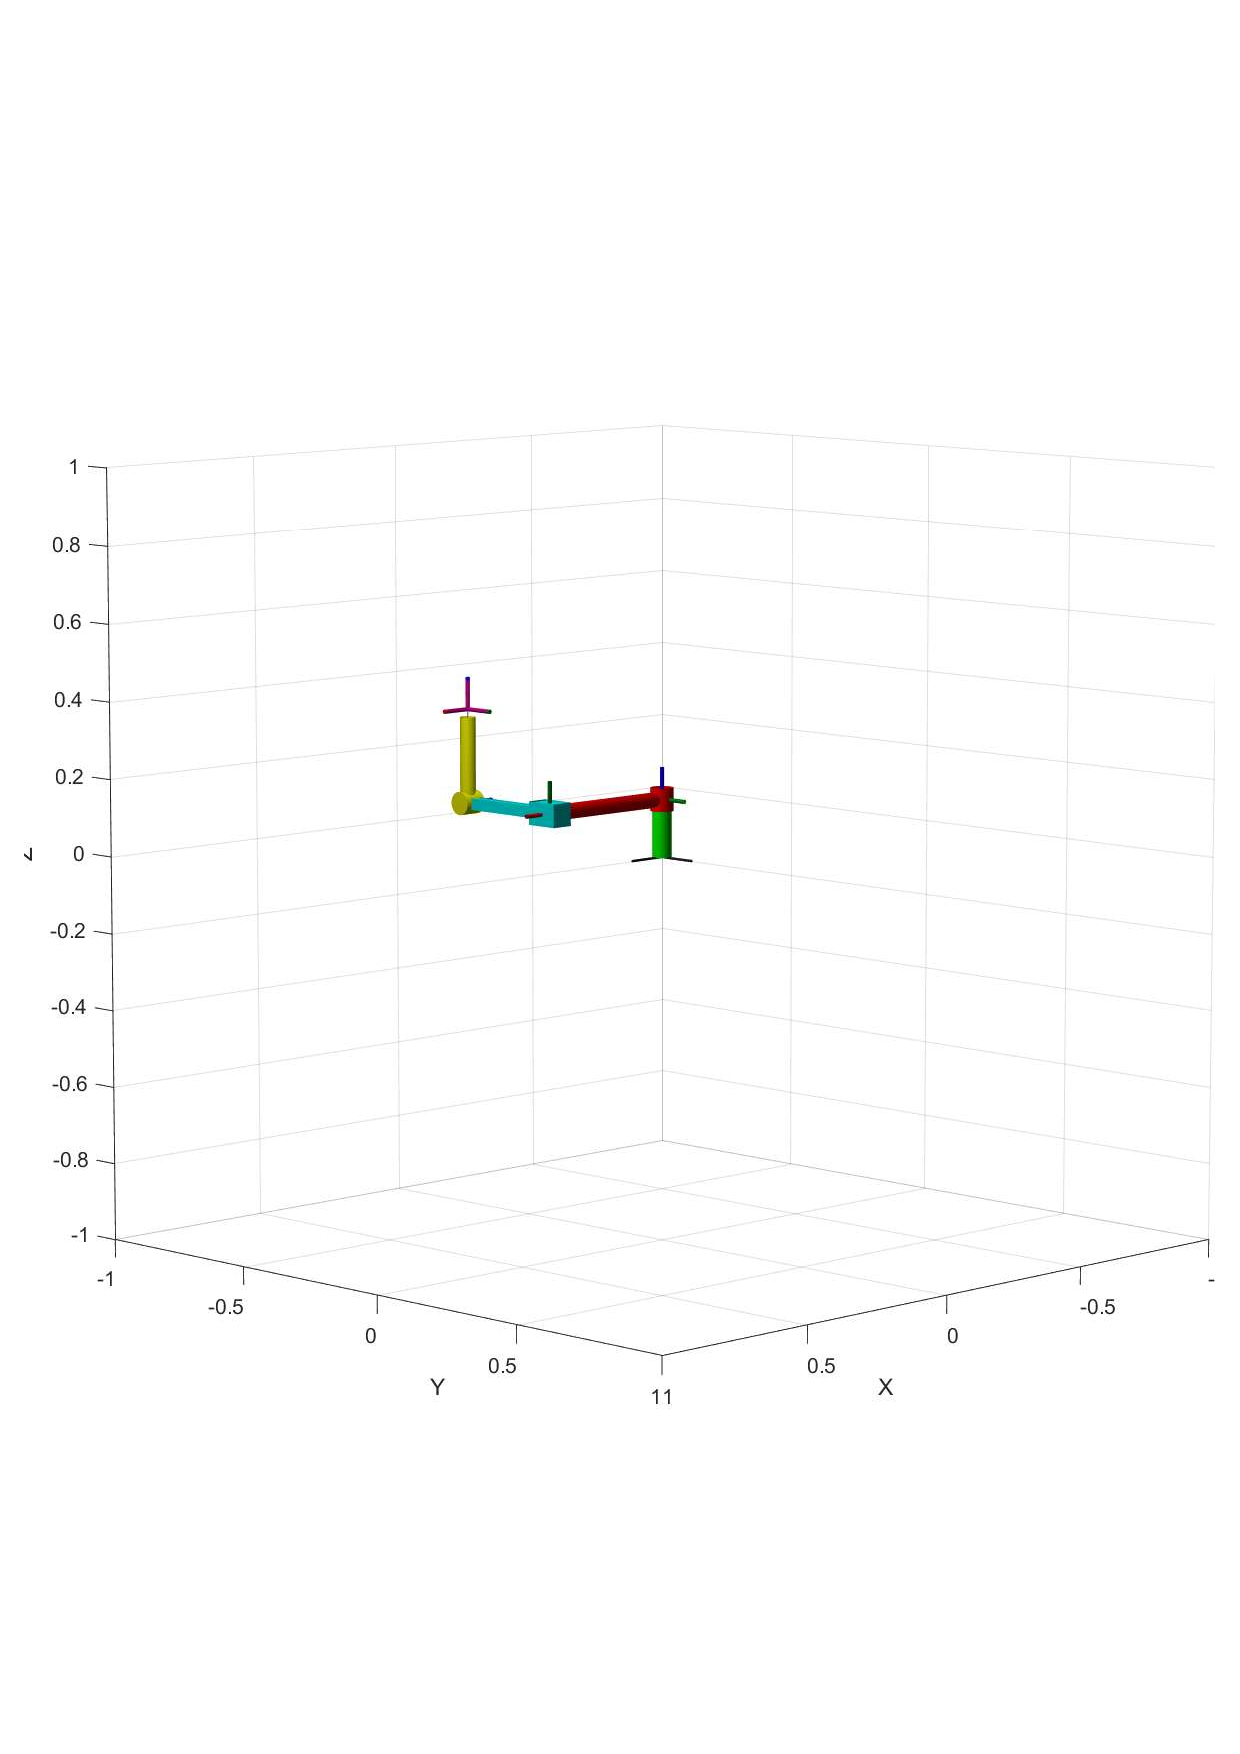
\includegraphics[width=0.70\textwidth]{figures/robot.pdf}
    \caption{3-DOF Robot Manipulator}
    \label{fig:robot_manipulator}
\end{figure}



\subsection{DH table}
The Denavit-Hartenberg (DH) parameters are used to describe the kinematics of a robot manipulator.
The DH parameters are four values that describe the relationship between two consecutive links in a robot manipulator.
The four values are: $a_i$, $d_i$, $\alpha_i$ and $\theta_i$. The $a_i$ and $d_i$ values are the lengths of the common normal and the link offset, respectively.
The $\alpha_i$ and $\theta_i$ values are the twist angle and the joint angle, respectively.
The DH table is a matrix that contains the DH parameters for each link in the robot manipulator.

\begin{table}[H]
    \centering
    \caption{DH Table}
    \renewcommand{\arraystretch}{1.5} % Increase the row height
    \begin{tabular}{|c|c|c|c|c|c|}
        \hline
        Frame              & Link & $a_i$ & $\alpha_i$       & $d_i$       & $\theta_i$                 \\ \hline
        $b \rightarrow 0$  &      & $0$   & 0                & $l_b$       & $0$                        \\ \hline
        $0 \rightarrow 1$  & 1    & $l_1$ & $\frac{\pi}{2}$  & 0           & $\theta_1$                 \\ \hline
        $1 \rightarrow 2$  & 2    & $0$   & $-\frac{\pi}{2}$ & $d_2 + 0.3$ & $\frac{\pi}{2}$            \\ \hline
        $2 \rightarrow 3$  & 3    & $l_3$ & 0                & 0           & $\theta_3 - \frac{\pi}{2}$ \\ \hline
        $3 \rightarrow ee$ &      & $0$   & $\frac{\pi}{2}$  & 0           & $\frac{\pi}{2}$            \\ \hline
    \end{tabular}
\end{table}


\subsection{Forward kinematics}
The forward kinematics is the process of determining the position and orientation of the end-effector of a robot manipulator given the joint angles.
The forward kinematics can be calculated using the DH parameters and the homogeneous transformation matrices.
The homogeneous transformation matrix is a 4x4 matrix that describes the relationship between two consecutive links in a robot manipulator.

The homogeneous transformation matrix between two consecutive links $i$ and $i+1$ is given by:
\begin{equation}
    T_{i,i+1} =
    \begin{bmatrix}
        c_{\theta_i} & -s_{\theta_i}c_{\alpha_i} & s_{\theta_i}s_{\alpha_i}  & a_i c_{\theta_i} \\
        s_{\theta_i} & c_{\theta_i}c_{\alpha_i}  & -c_{\theta_i}s_{\alpha_i} & a_i s_{\theta_i} \\
        0            & s_{\alpha_i}              & c_{\alpha_i}              & d_i              \\
        0            & 0                         & 0                         & 1                \\
    \end{bmatrix}
\end{equation}

The forward kinematics can be calculated by multiplying the homogeneous transformation matrices for each link in the robot manipulator.
The forward kinematics can be calculated using the following equation:

\begin{equation}
    T_{b,ee} = T_{b,0} \times T_{0,1} \times T_{1,2} \times T_{2,3} \times T_{3,ee}
\end{equation}

Where $T_{b,ee}$ is the homogeneous transformation matrix between the base frame and the end-effector frame (accordingly to the nsa convention):
\begin{equation}
    \renewcommand{\arraystretch}{1.5} % Increase the row height
    \resizebox{\textwidth}{!}{
        $T_{b,ee} = \left(\begin{array}{cccc}
                    -\sin\left(\theta _{1}\right)\,\sin\left(\theta _{3}\right) & -\cos\left(\theta _{1}\right) & \cos\left(\theta _{3}\right)\,\sin\left(\theta _{1}\right)  & \frac{2\,\cos\left(\theta _{1}\right)}{5}+\frac{3\,\sin\left(\theta _{1}\right)}{10}+\frac{6\,\cos\left(\theta _{3}\right)\,\sin\left(\theta _{1}\right)}{25}+\theta _{2}\,\sin\left(\theta _{1}\right) \\
                    \cos\left(\theta _{1}\right)\,\sin\left(\theta _{3}\right)  & -\sin\left(\theta _{1}\right) & -\cos\left(\theta _{1}\right)\,\cos\left(\theta _{3}\right) & \frac{2\,\sin\left(\theta _{1}\right)}{5}-\frac{3\,\cos\left(\theta _{1}\right)}{10}-\frac{6\,\cos\left(\theta _{1}\right)\,\cos\left(\theta _{3}\right)}{25}-\theta _{2}\,\cos\left(\theta _{1}\right) \\
                    \cos\left(\theta _{3}\right)                                & 0                             & \sin\left(\theta _{3}\right)                                & \frac{6\,\sin\left(\theta _{3}\right)}{25}+\frac{3}{20}                                                                                                                                                 \\
                    0                                                           & 0                             & 0                                                           & 1
                \end{array}\right)$
    }
\end{equation}


For all the others matrices see the matlab code.






\subsection{Inverse kinematics}
\justify
The inverse kinematics is the process of determining the joint angles of a robot manipulator given the position and orientation of the end-effector.
The inverse kinematics can be calculated using the DH parameters and the homogeneous transformation matrices, and we can start from the following equation:

\begin{equation}
    \renewcommand{\arraystretch}{1.5}
    T_e ^b =
    \begin{bmatrix}
        \frac{2}{5} \cos \theta_1 + \frac{3}{10} \sin \theta_1 + \frac{6}{25} \cos \theta_3 \sin \theta_1 + \theta_2 \sin \theta_1 \\
        \frac{2}{5} \sin \theta_1 - \frac{3}{10} \cos \theta_1 - \frac{6}{25} \cos \theta_3 \cos \theta_1 - \theta_2 \cos \theta_1 \\
        \frac{6}{25} \sin \theta_3 + \frac{3}{20}
    \end{bmatrix}
\end{equation}

From the last row of the matrix, we can find the value of $\theta_3$:
\begin{equation}
    \theta_3 = \arcsin \left( \frac{z-0.15}{0.24}\right)
\end{equation}

Then, if we apply the technique of summing the squares of the first two rows, we can find the value of $\theta_2$:


\begin{equation}
    \theta_2 = \frac{-0.6 \pm \sqrt{-0.6^2 - 4 (\frac{53}{50} - x^2 - y^2)}}{2}
\end{equation}

Finally, we can find the value of $\theta_1$ by substituting the values of $\theta_2$ and $\theta_3$ in the first row of the matrix and recalling the Weierstrass substitution formulas:

\begin{equation}
    \sin x = \frac{2t}{1+t^{2}}
\end{equation}
\begin{equation}
    \cos x = \frac{1-t^{2}}{1+t^{2}}
\end{equation}
\begin{equation}
    x = \tan \frac{x}{2}
\end{equation}

\begin{equation}
    \theta_1 = \frac{2A \pm \sqrt{4A^2 - 4 (x-2)^2}}{2 (x-2)}
\end{equation}

where A is:
\begin{equation}
    A = 0.3+\frac{6}{25} \cos \theta_3 + \theta_2
\end{equation}




\subsection{Geometric Jacobian}

The geometric Jacobian matrix is a 6x3 matrix that describes the relationship between the joint velocities and the end-effector velocities of a robot manipulator.

The geometric Jacobian matrix can be calculated using the following equation:

\begin{equation}
    \renewcommand{\arraystretch}{1.5} % Increase the row height
    \resizebox{\textwidth}{!}{
        $J_{geometric} = \begin{pmatrix}
                \frac{3\,\cos\left(\theta _{1}\right)}{10}-\frac{2\,\sin\left(\theta _{1}\right)}{5}+\frac{6\,\cos\left(\theta _{1}\right)\,\cos\left(\theta _{3}\right)}{25}+\theta _{2}\,\cos\left(\theta _{1}\right) & \sin\left(\theta _{1}\right)  & -\frac{6\,\sin\left(\theta _{1}\right)\,\sin\left(\theta _{3}\right)}{25} \\
                \frac{2\,\cos\left(\theta _{1}\right)}{5}+\frac{3\,\sin\left(\theta _{1}\right)}{10}+\frac{6\,\cos\left(\theta _{3}\right)\,\sin\left(\theta _{1}\right)}{25}+\theta _{2}\,\sin\left(\theta _{1}\right) & -\cos\left(\theta _{1}\right) & \frac{6\,\cos\left(\theta _{1}\right)\,\sin\left(\theta _{3}\right)}{25}  \\
                0                                                                                                                                                                                                       & 0                             & \frac{6\,\cos\left(\theta _{3}\right)}{25}                                \\
                0                                                                                                                                                                                                       & 0                             & -\cos\left(\theta _{1}\right)                                             \\
                0                                                                                                                                                                                                       & 0                             & -\sin\left(\theta _{1}\right)                                             \\
                1                                                                                                                                                                                                       & 0                             & 0
            \end{pmatrix}$
    }
\end{equation}


\subsection{Analytical Jacobian}

The analytical Jacobian matrix is a 6x3 matrix and it's calculated as the derivative of the forward kinematics with respect to the joint angles.
The analytical Jacobian matrix can be calculated using the following equation:

\begin{equation}
    \renewcommand{\arraystretch}{1.5} % Increase the row height
    \resizebox{\textwidth}{!}{
        $J_{analytical} = \left(\begin{array}{ccc}
                    \frac{3\,\cos\left(\theta _{1}\right)}{10}-\frac{2\,\sin\left(\theta _{1}\right)}{5}+\frac{6\,\cos\left(\theta _{1}\right)\,\cos\left(\theta _{3}\right)}{25}+\theta _{2}\,\cos\left(\theta _{1}\right) & \sin\left(\theta _{1}\right)  & -\frac{6\,\sin\left(\theta _{1}\right)\,\sin\left(\theta _{3}\right)}{25}       \\
                    \frac{2\,\cos\left(\theta _{1}\right)}{5}+\frac{3\,\sin\left(\theta _{1}\right)}{10}+\frac{6\,\cos\left(\theta _{3}\right)\,\sin\left(\theta _{1}\right)}{25}+\theta _{2}\,\sin\left(\theta _{1}\right) & -\cos\left(\theta _{1}\right) & \frac{6\,\cos\left(\theta _{1}\right)\,\sin\left(\theta _{3}\right)}{25}        \\
                    0                                                                                                                                                                                                       & 0                             & \frac{6\,\cos\left(\theta _{3}\right)}{25}                                      \\
                    1                                                                                                                                                                                                       & 0                             & 0                                                                               \\
                    0                                                                                                                                                                                                       & 0                             & -\frac{\cos\left(\theta _{3}\right)}{\left|\cos\left(\theta _{3}\right)\right|} \\
                    0                                                                                                                                                                                                       & 0                             & 0
                \end{array}\right)$
    }
\end{equation}





\section{Second homework: Kinetic and potential energy}
\justify
\subsection{Kinetic energy}
The kinetic energy of a robot manipulator is the energy due to the motion of the robot.
Before calculating the kinetic energy, we need to calculate the partial jacobian for every joint, as shown in the following equation:
\begin{equation}
    \sum_{i=1}^{n} \left( m_{\ell_i} \left( J_P^{\ell_i} \right)^T J_P^{\ell_i} + \left( J_O^{\ell_i} \right)^T R_i I_{\ell_i}^i R_i^T J_O^{\ell_i} \right)
\end{equation}

In particular, the partial jacobian for the end effector is given by:

positional part:
\begin{equation}
    j_{P_j}^{l_i} =
    \begin{cases}
        Z_{j-1},                            & \text{prismatic joint} \\
        Z_{j-1} \times (p_{l_i} - p_{j-1}), & \text{revolute joint}
    \end{cases}
\end{equation}

rotational part:
\begin{equation}
    j_{Oj}^{l_i} =
    \begin{cases}
        0,       & \text{prismatic joint} \\
        Z_{j-1}, & \text{revolute joint}
    \end{cases}
\end{equation}


where
\begin{itemize}
    \item $p_{j-1}$ is the position vector of the origin of Frame $\Sigma_{j-1}$ w.r.t. $\Sigma_0$
    \item $z_{j-1}$ is the unit vector of axis $z$ of Frame $\Sigma_{j-1}$ w.r.t. $\Sigma_0$
\end{itemize}

Now, we need and additional matrix, the inertia matrix for each link, wrt the frame attached to the current link. \\
To compute this matrix we also use \textbf{Steiner's theorem}, which states that the inertia matrix of a body with respect to a point $P$ is equal to the inertia matrix of the body with respect to its center of mass $G$
plus the mass of the body times the square of the distance between $G$ and $P$ times the identity matrix.

for prismatics joints the inertia matrix wrt to the CoM is the following:

\begin{equation}
    I_C = \begin{bmatrix}
        \frac{1}{12}m(b^2 + c^2) & 0                        & 0                        \\
        0                        & \frac{1}{12}m(a^2 + c^2) & 0                        \\
        0                        & 0                        & \frac{1}{12}m(a^2 + b^2)
    \end{bmatrix}
\end{equation}

Remapping the inertia matrix to the frame of the link, we obtain:
\begin{align}
    I & = I_C + m \left( \begin{bmatrix} -\frac{a}{2} & 0 & 0 \end{bmatrix} \begin{bmatrix} -\frac{a}{2} \\ 0 \\ 0 \end{bmatrix} I_{3 \times 3} \right. \nonumber
      & \quad \left. - \begin{bmatrix} -\frac{a}{2} \\ 0 \\ 0 \end{bmatrix} \begin{bmatrix} -\frac{a}{2} & 0 & 0 \end{bmatrix} \right) =                          \\
      & = \begin{bmatrix}
              0.0151 & 0      & 0      \\
              0      & 0.0601 & 0      \\
              0      & 0      & 0.0453
          \end{bmatrix}
\end{align}


for revolute joints:

\begin{equation}
    I_C = \begin{bmatrix}
        \frac{1}{2}m(a^2 + b^2) & 0                                  & 0                                  \\
        0                       & \frac{1}{2}m(3(a^2 + b^2)^2 + h^2) & 0                                  \\
        0                       & 0                                  & \frac{1}{2}m(3(a^2 + b^2)^2 + h^2)
    \end{bmatrix}
\end{equation}

Remapping the inertia matrix to the frame of the link, we obtain:

\begin{align}
    I & = I_C + m \left( \begin{bmatrix} -\frac{h}{2} & 0 & 0 \end{bmatrix} \begin{bmatrix} -\frac{h}{2} \\ 0 \\ 0 \end{bmatrix} I_{3 \times 3} - \begin{bmatrix} -\frac{h}{2} \\ 0 \\ 0 \end{bmatrix} \begin{bmatrix} -\frac{h}{2} & 0 & 0 \end{bmatrix} \right) = \nonumber \\
      & = \begin{bmatrix}
              0.0004 & 0      & 0      \\
              0      & 0.2400 & 0      \\
              0      & 0      & 0.2400
          \end{bmatrix} and
    \begin{bmatrix}
        0.0004 & 0      & 0      \\
        0      & 0.0864 & 0      \\
        0      & 0      & 0.0864
    \end{bmatrix}
\end{align}

Finally, we can calculate the kinetic energy of the robot manipulator using the following equation:

All the computations are made with symbolic toolbox in Matlab, and to obtain a numerical value we need to substitute the values for the joints and velocities.
In this specific case, we choose the following values:
\\

jointValues = $[\frac{\pi}{2}, -0.2, \frac{\pi}{3}]$ \\

velocityValues = $[5, 2, 8]$ \\

accelerationValues = $[4, 1, 2]$

\begin{equation}
    K =  \frac{1}{2} \dot{q}^T \left[ \sum_{i=1}^{n} \left( m_{l_i} (J_P^{l_j})^T J_P^{l_i} + (J_O^{l_i})^T R_i I_{l_i}^{i} R_i^T J_O^{l_i} \right) \right] \dot{q} =  8.8520 J
\end{equation}

Where the part inside the square brakets is the inertia matrix of the robot, and it's called $B$.



\subsection{Potential energy}

Regarding the potential energy, it's way easier to compute, since it's just the sum of the potential energy of each link, which is given by:

\begin{equation}
    \mathcal{U} = \sum_{i=1}^{n} \mathcal{U}_i = - \sum_{i=1}^{n} m_{l_i} g_0^T \rho_{l_i} =    10.8680 J
\end{equation}

Recalling that the gravity vector is $g_0 = [0, 0, -9.81]$.


\section{Third homework: Equations of motion}
\justify

\subsection{$\tau$ with derivatives}

The lagrangian of a system is defined as the sum between the kinetic energy and the potential energy of the system.
\begin{equation}
    \mathcal{L}(q, \dot{q}) = \mathcal{T}(q, \dot{q}) - \mathcal{U}(q) = \frac{1}{2} \dot{q}^T B(q) \dot{q} + \sum_{i=1}^{n} m_{l_i} g_0^T \rho_{l_i}
\end{equation}

Now, to obtain the $tau$, the torques to be imparted to the robot's motors, we must calculate the derivative of the Lagrangian, first with respect to $dot{q}$ and then with respect to $q$.
\begin{equation}
    \left( \frac{\partial \mathcal{L}}{\partial \dot{q}} \right)^T = B(q) \dot{q}
\end{equation}

\begin{equation}
    \left( \frac{\partial \mathcal{L}}{\partial \dot{q}} \right)^T = \frac{1}{2} \left( \frac{\partial}{\partial \dot{q}} \left( \dot{q}^T B(q) \dot{q} \right) \right)^T - \left( \frac{\partial \mathcal{U}}{\partial q} \right)^T
\end{equation}

\begin{equation}
    \frac{d}{dt} \left( \frac{\partial \mathcal{L}}{\partial \dot{q}} \right)^T = B(q) \ddot{q} + \dot{B}(q) \dot{q}
\end{equation}


If we substitute the values for the joints, elocities and acceleration, we obtain the following values for the torques:
\begin{equation}
    \tau = \begin{bmatrix}
        4.6117   \\
        -15.9957 \\
        3.2947
    \end{bmatrix}
\end{equation}

\subsection{$\tau$ without derivatives}

If we don's want to compute all this derivatives, we have an other way to compute the torques, using the Coriolis and centrifugal matrices and the gravity vector.
As we'll see the results for the torques are the same.

\begin{equation}
    \sum_{j=1}^{n} b_{ij}(q) \ddot{q}_j + \sum_{j=1}^{n} c_{ij}(q, \dot{q}) \dot{q}_j + g_i(q) = \tau_i
\end{equation}

where the gravity vector is given by:

\begin{equation}
    \sum_{j=1}^{n} m_{l_j} g_0^T J_{Pi}^{l_j}(q)
\end{equation}


and the $c_i,_j$ terms is given by:

\begin{equation}
    \sum_{j=1}^{n} \sum_{k=1}^{n} h_{ijk}(q) \dot{q}_k \dot{q}_j
\end{equation}


After all the computations in Matlab, that are too long to be written here, we obtain the following values for the torques:
\begin{equation}
    \tau = \begin{bmatrix}
        4.6117   \\
        -15.9957 \\
        3.2947
    \end{bmatrix}
\end{equation}

that are exactly the same as the ones obtained with the derivatives of the Lagrangian.




\section{Fourth homework: Newton-Euler formulation}
\justify

The NE formulation is based on the balance of all the forces acting on the generic link of
the manipulator. It's divided in two steps: the first one is the forward dynamics, where we compute the linear and angular velocities and accelerations of the links, and the second one is the backward dynamics, where we compute the torques to be imparted to the motors.
It's important to remember that the NE formulation is an algorithmic and numerical method, and it's not as precise as the Lagrangian formulation, but it's much faster and easier to compute.

Before starting with the computations, we need to understand what is the augmented link, which is the link that we are studying in the current iteration of the algorithm plus the mass of the motor and the inertia.



\subsection{Forward dynamics}

The forward recursion is performed for propagating link velocities and accelerations
from i = 0 to i = n.
For all the code see the Matlab code.

\subsection{Backward dynamics}

The backward recursion for propagating forces from i = n to i = 0.
For all the code see the Matlab code.

\vspace{1cm}
Finally, as expected, torques computed with the NE formulation are the same as the ones computed with the Lagrangian formulation.
In particular, we have the following values for the torques:

\begin{equation}
    \tau = \begin{bmatrix}
        4.6117   \\
        -15.9957 \\
        3.2947
    \end{bmatrix}
\end{equation}

when the joint values, velocities and accelerations are the following:
\\

jointValues = $[\frac{\pi}{2}, -0.2, \frac{\pi}{3}]$ \\

velocityValues = $[5, 2, 8]$ \\

accelerationValues = $[4, 1, 2]$




\section{Control Scheme}
\justify

\subsection{PD control law with gravity compensation in joint space}

\begin{figure}[H]
    \centering
    \makebox[\textwidth][c]{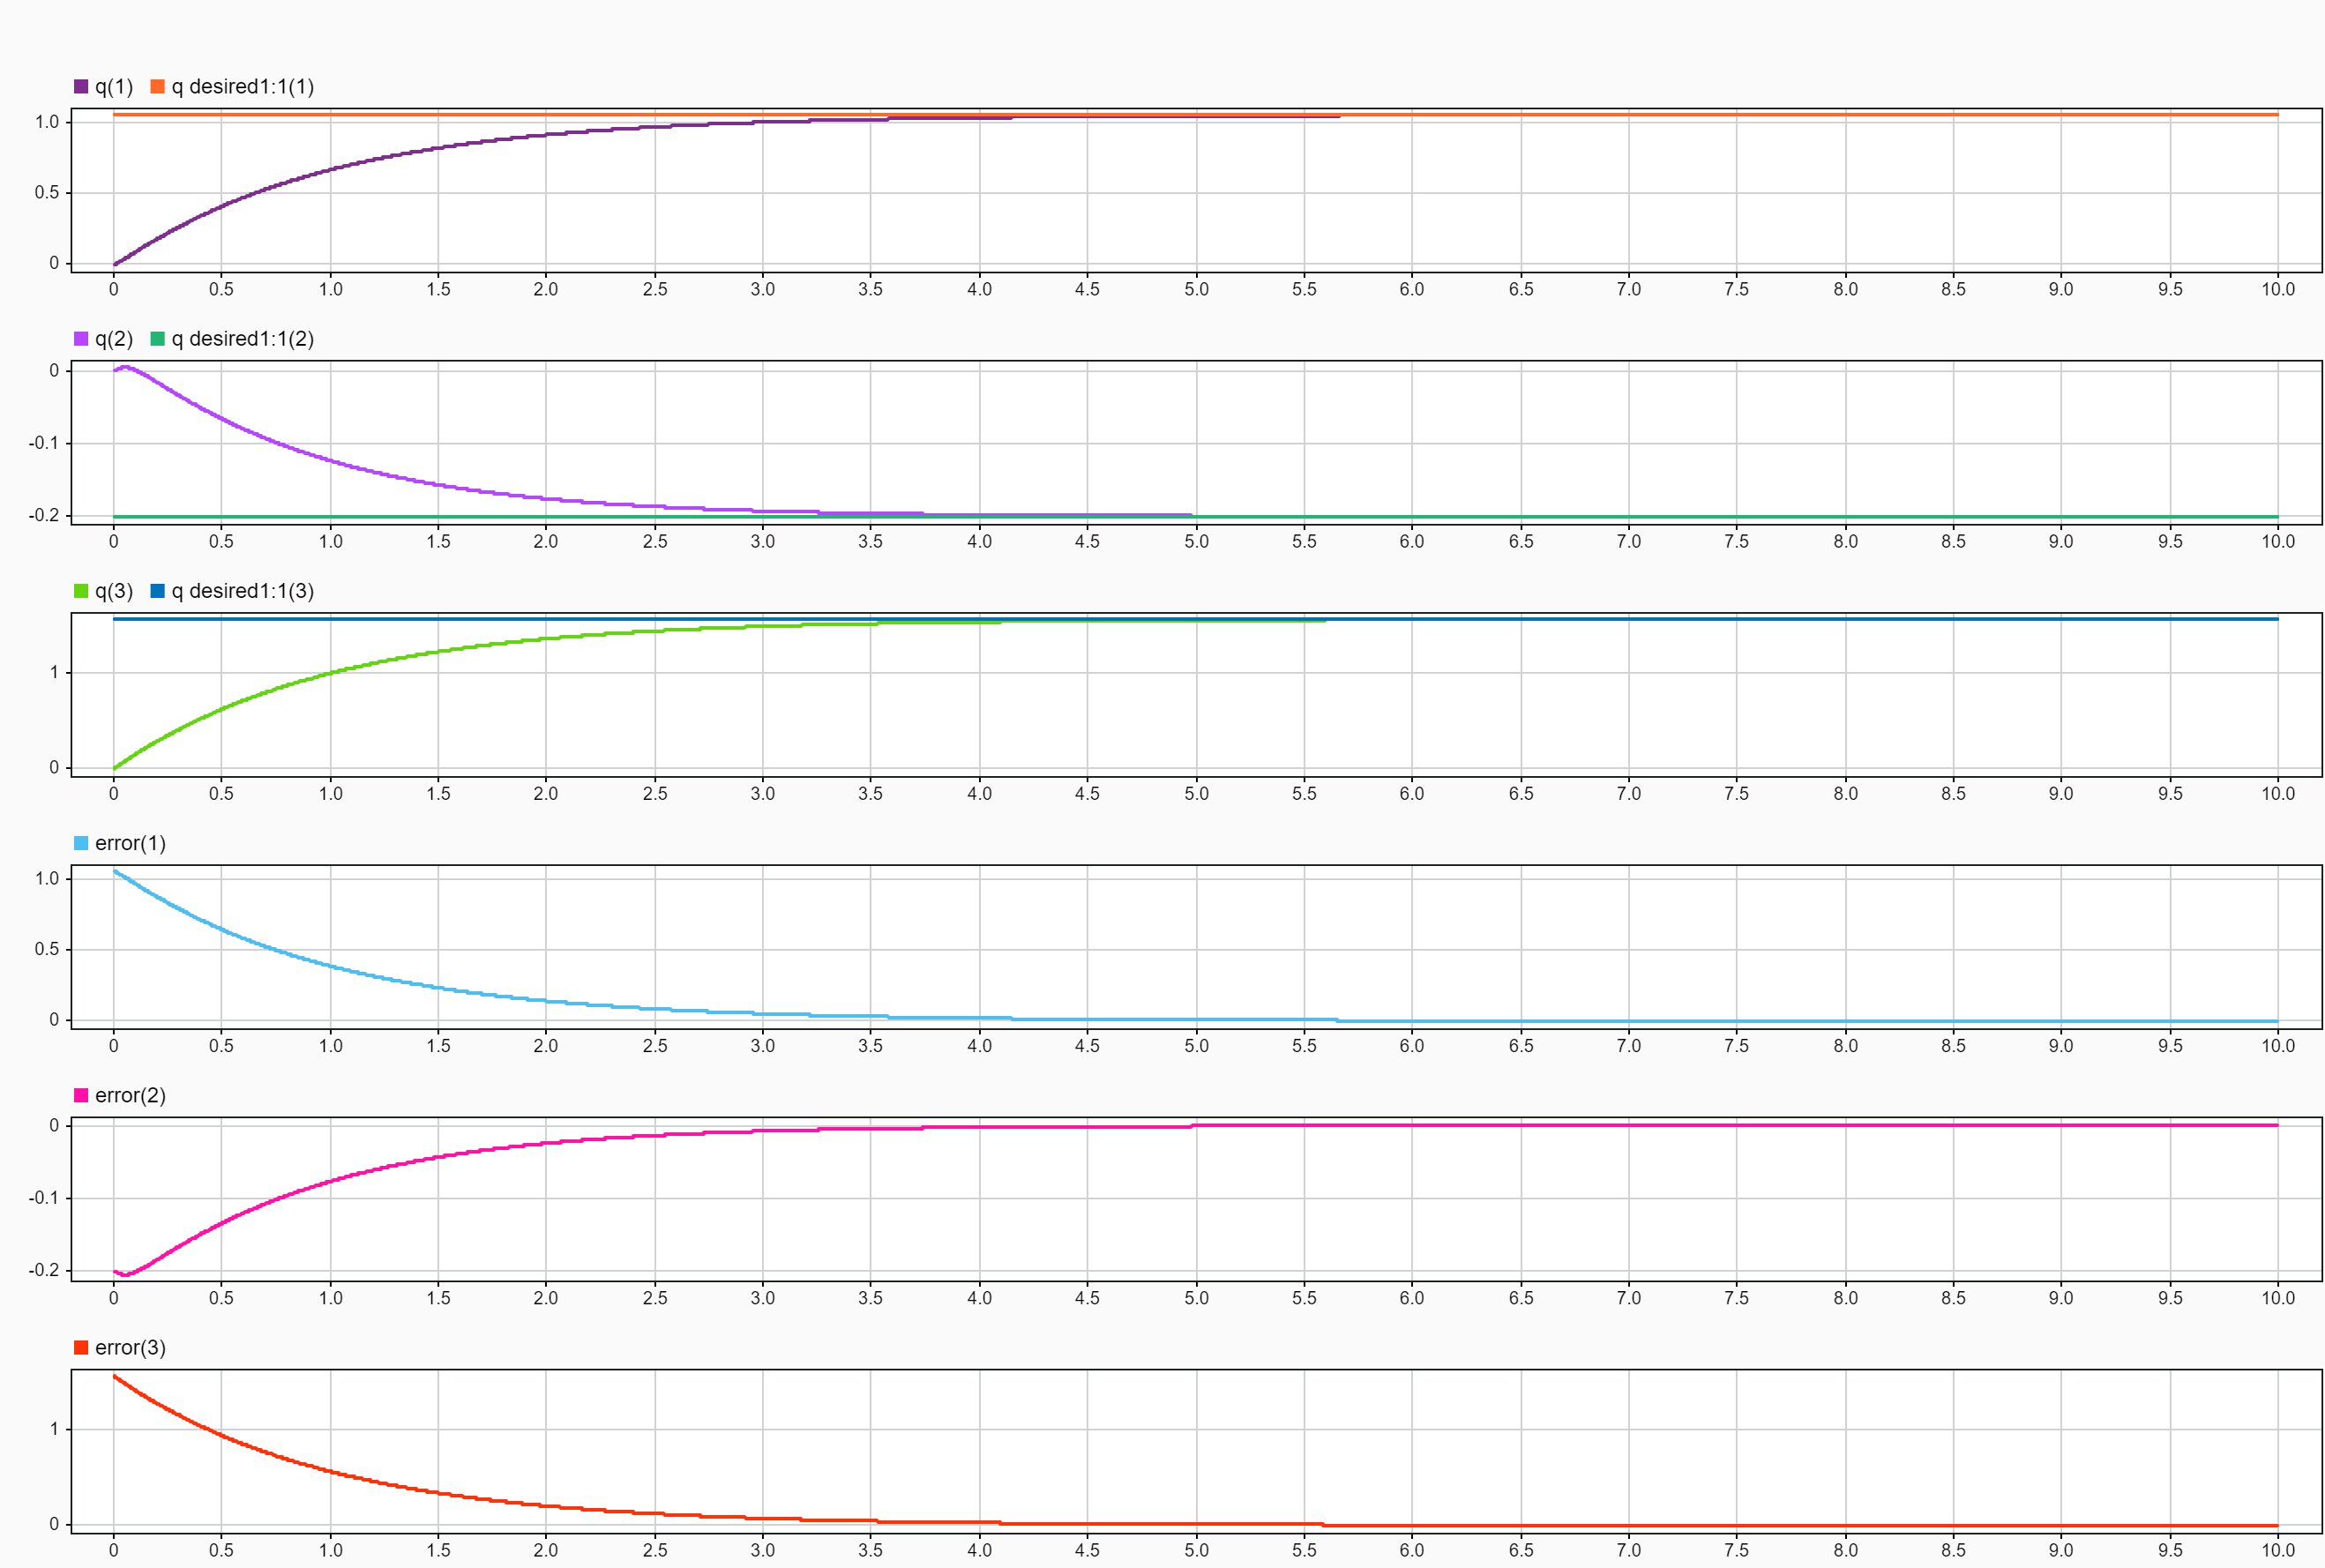
\includegraphics[width=1.6\textwidth]{../Simulink/Images/GravityCompensationControl.png}}
    \caption{PD control law with gravity compensation in joint space}
    \label{fig:PD control law with gravity compensation in joint space}
\end{figure}



\subsection{Inverse dynamic control law in joint space}

\begin{figure}[H]
    \centering
    \makebox[\textwidth][c]{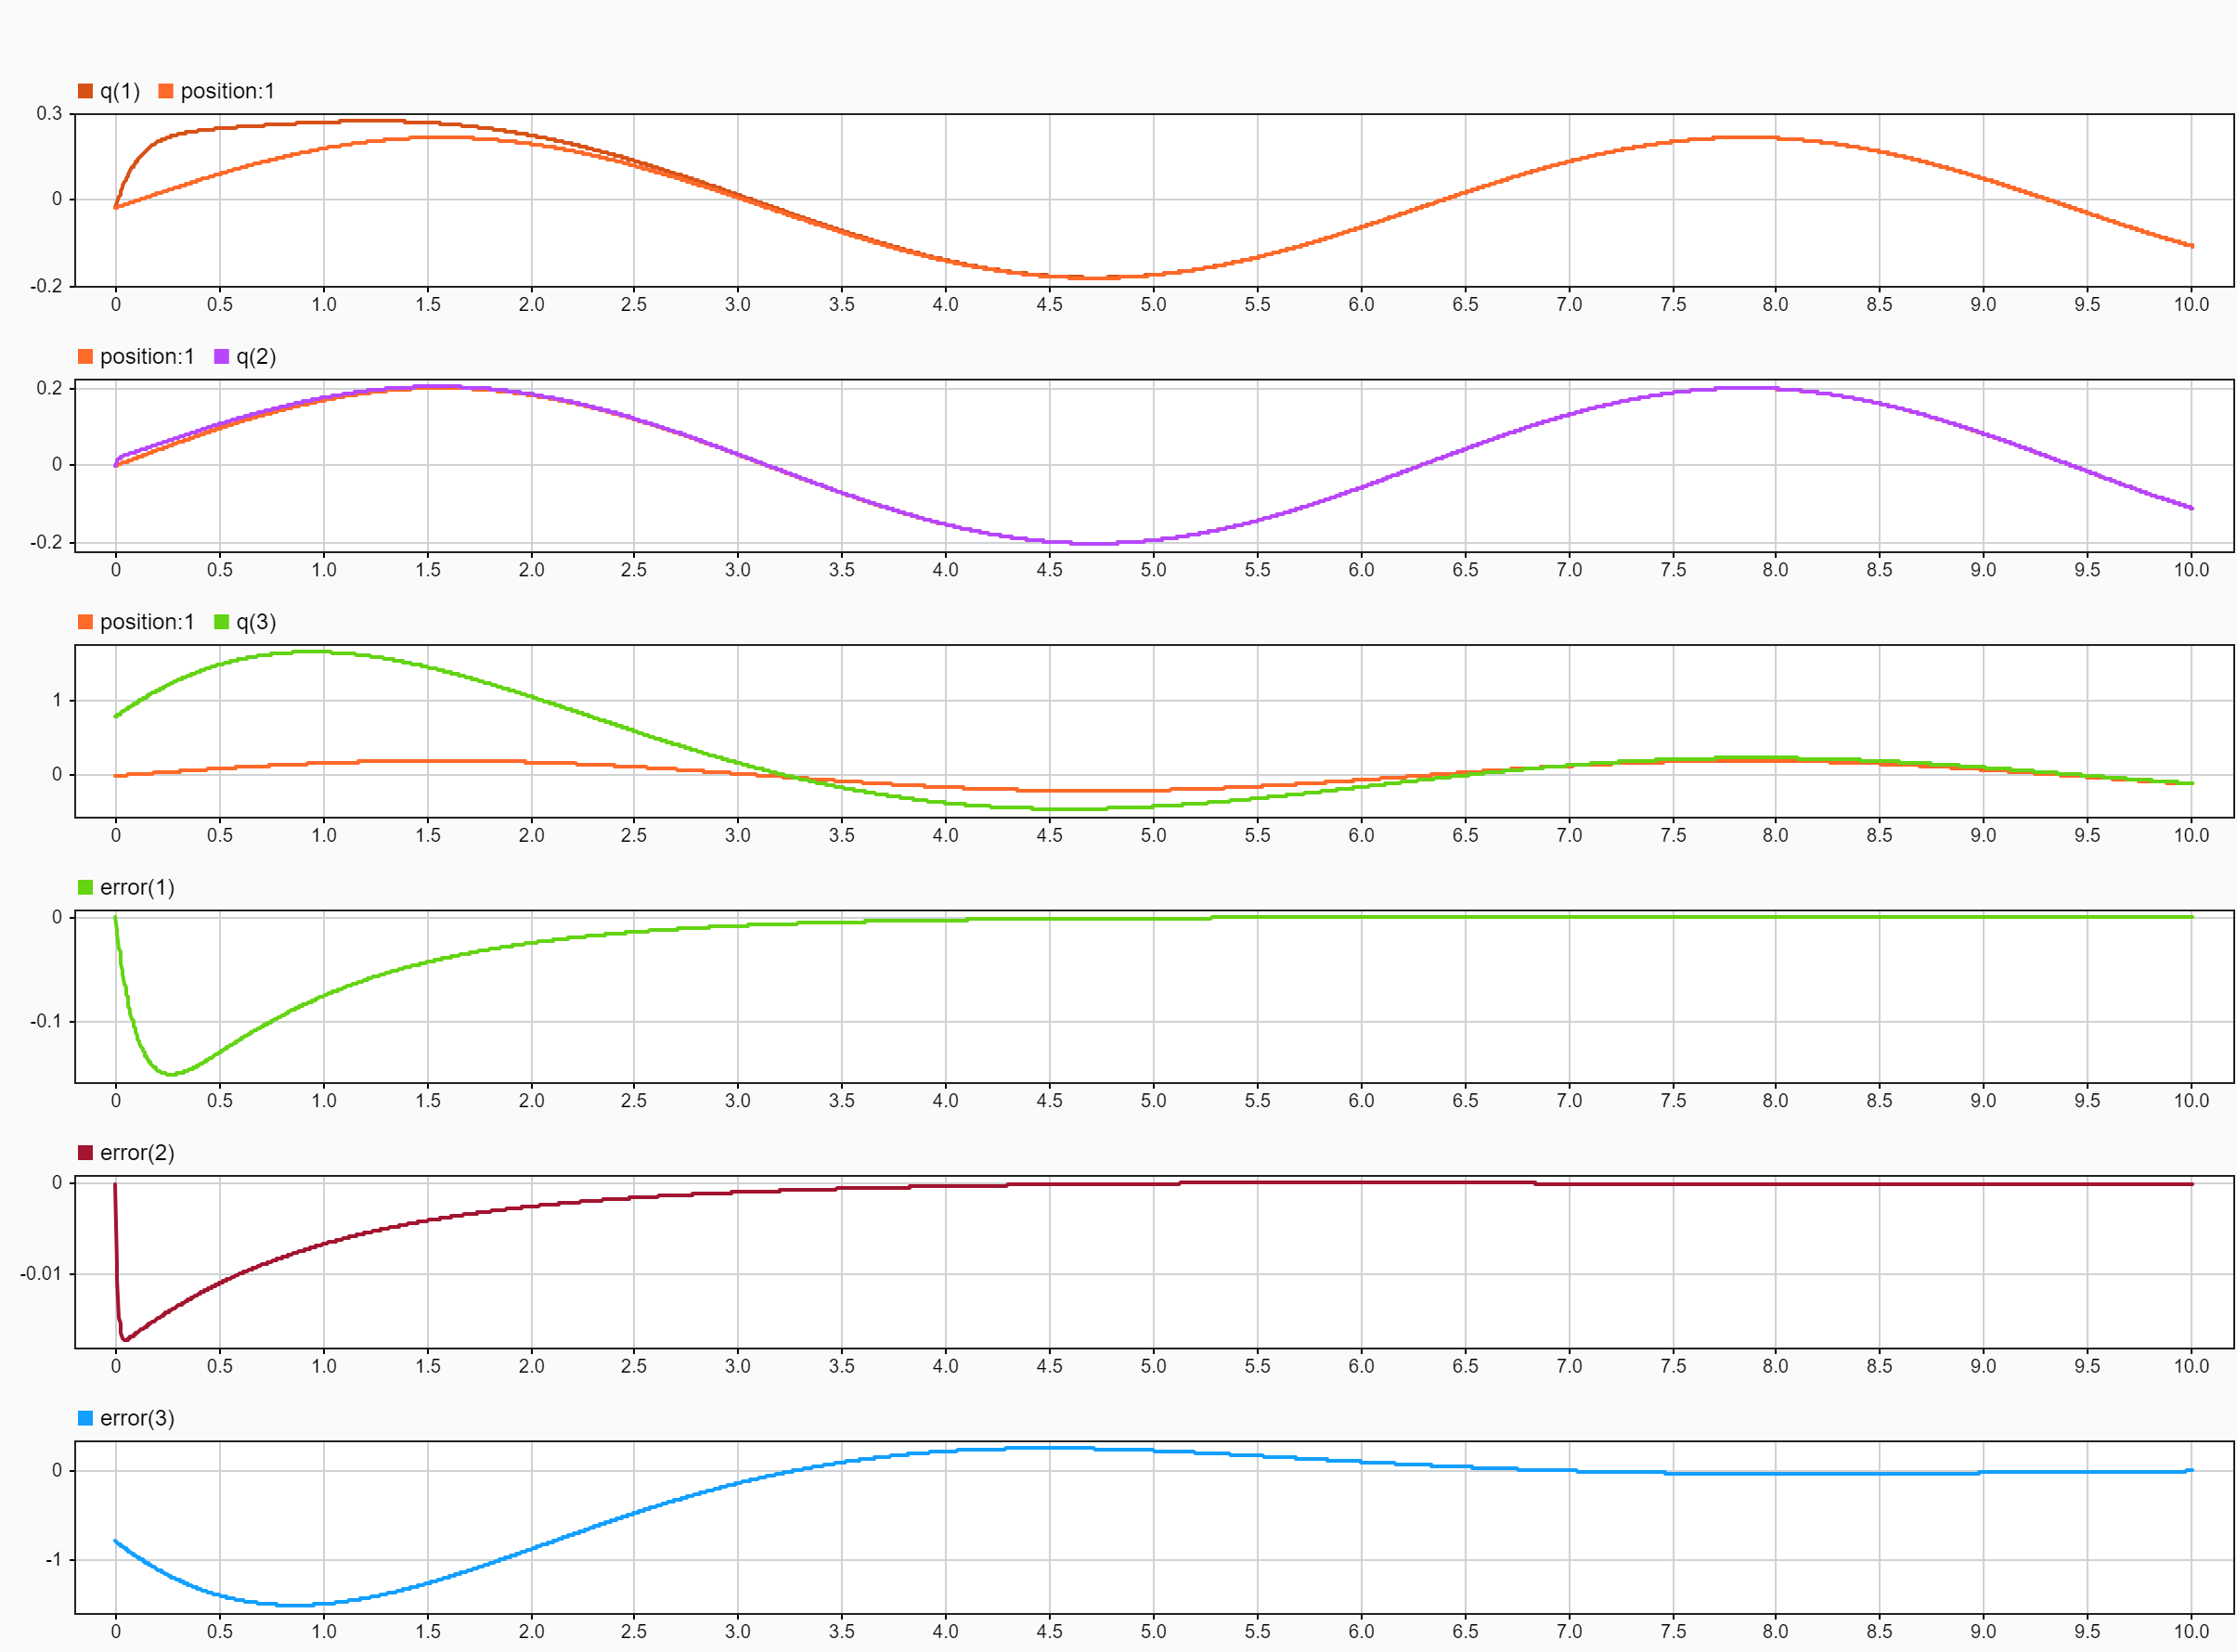
\includegraphics[width=1.6\textwidth]{../Simulink/Images/InverseDynamicControl.png}}
    \caption{Inverse dynamic control law in joint space}
    \label{fig:Inverse dynamic control law in joint space}
\end{figure}

\subsection{PD control law with gravity compensation in the operational space}
\begin{figure}[H]
    \centering
    \makebox[\textwidth][c]{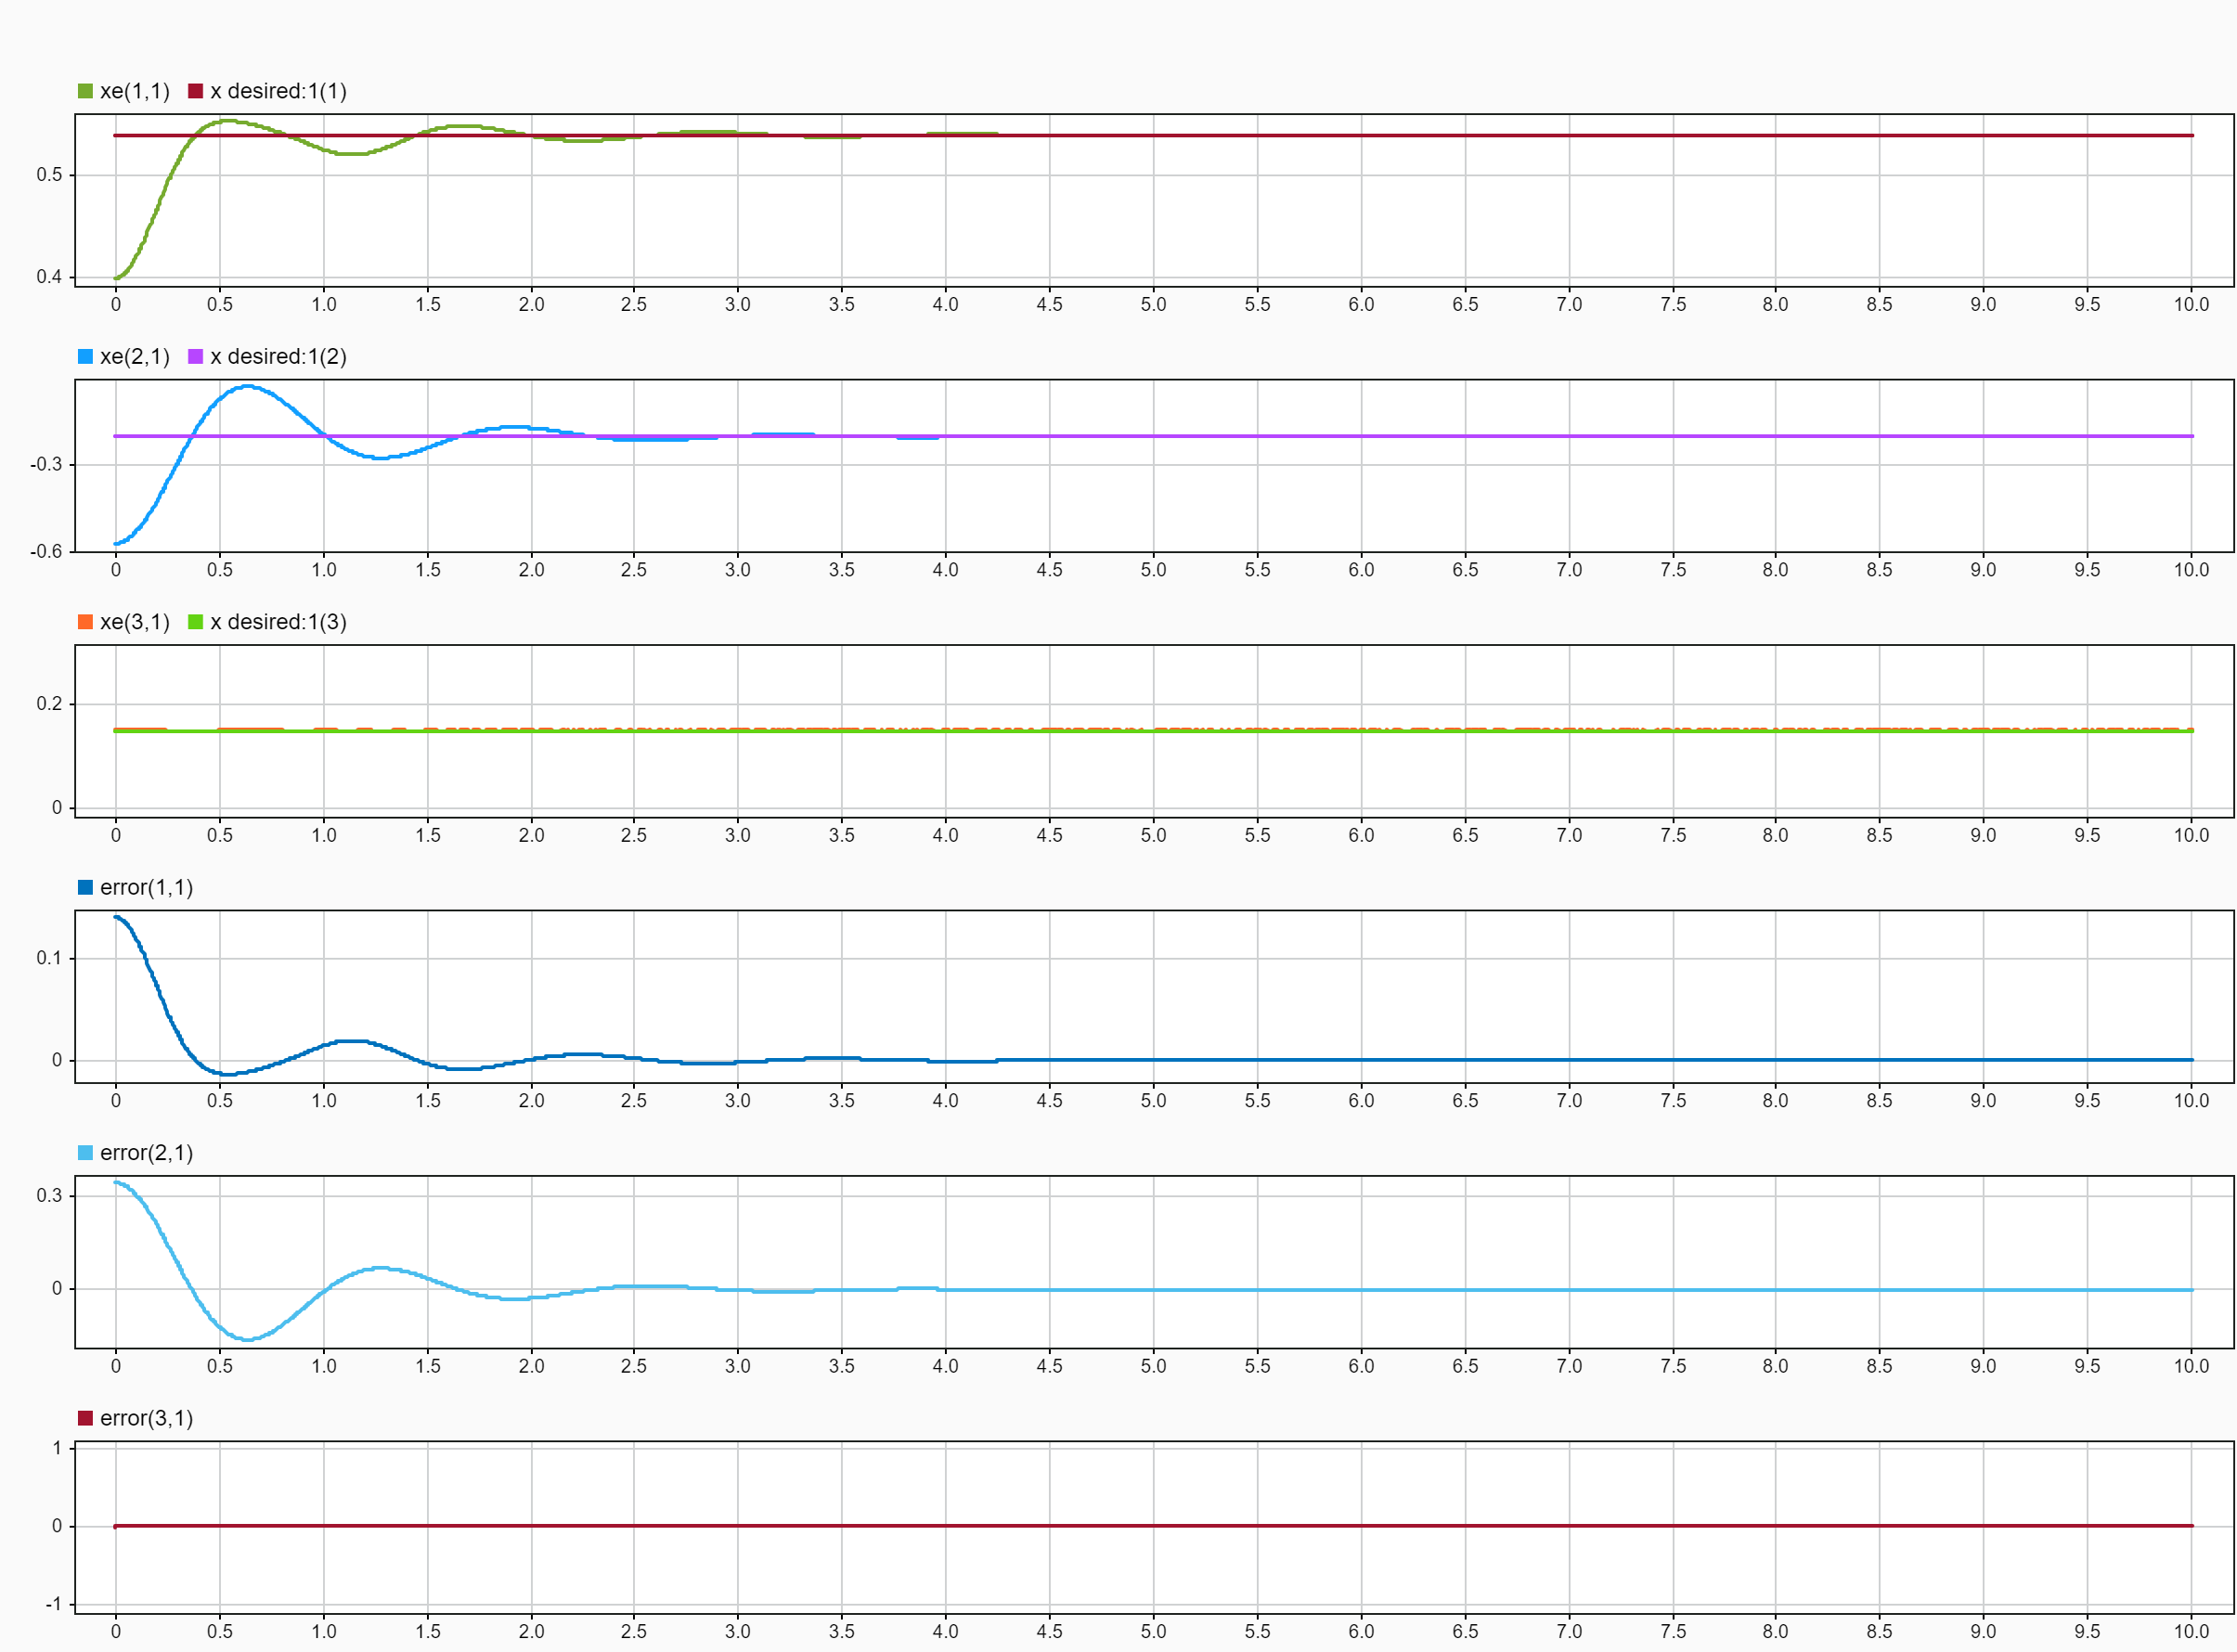
\includegraphics[width=1.6\textwidth]{../Simulink/Images/GravityCompensationControl_operationalSpace.png}}
    \caption{PD control law with gravity compensation in the operational space}
    \label{fig:PD control law with gravity compensation in the operational space}
\end{figure}




\subsection{Inverse dynamic control law in the operational space}

Here I study two different cases: the first one is the case where the robot can reach the configuration, and the second one is the case where the robot cannot reach the configuration.

In the first one we have:

\begin{figure}[H]
    \centering
    \makebox[\textwidth][c]{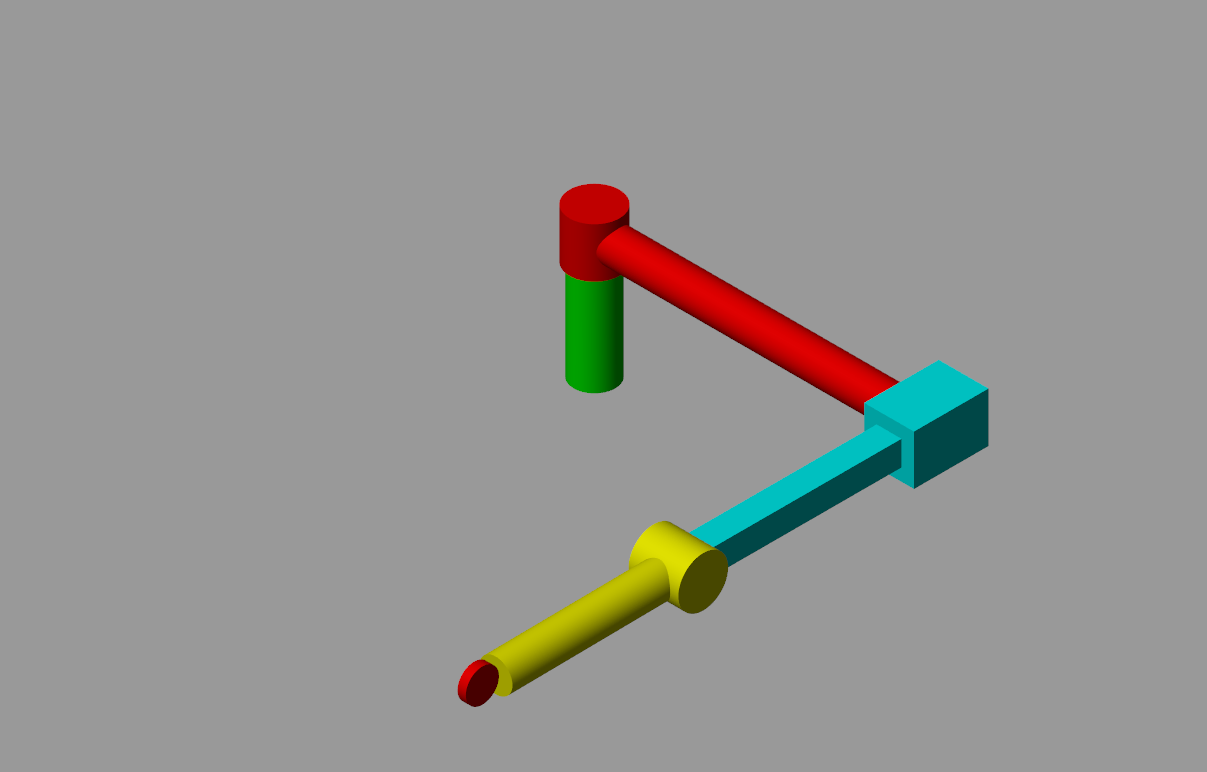
\includegraphics[width=0.6\textwidth]{../Simulink/Images/inverseDynamic2.png}}
    \caption{The robot can reach the position}
    \label{fig:The robot can reach the position}
\end{figure}


\begin{figure}[H]
    \centering
    \makebox[\textwidth][c]{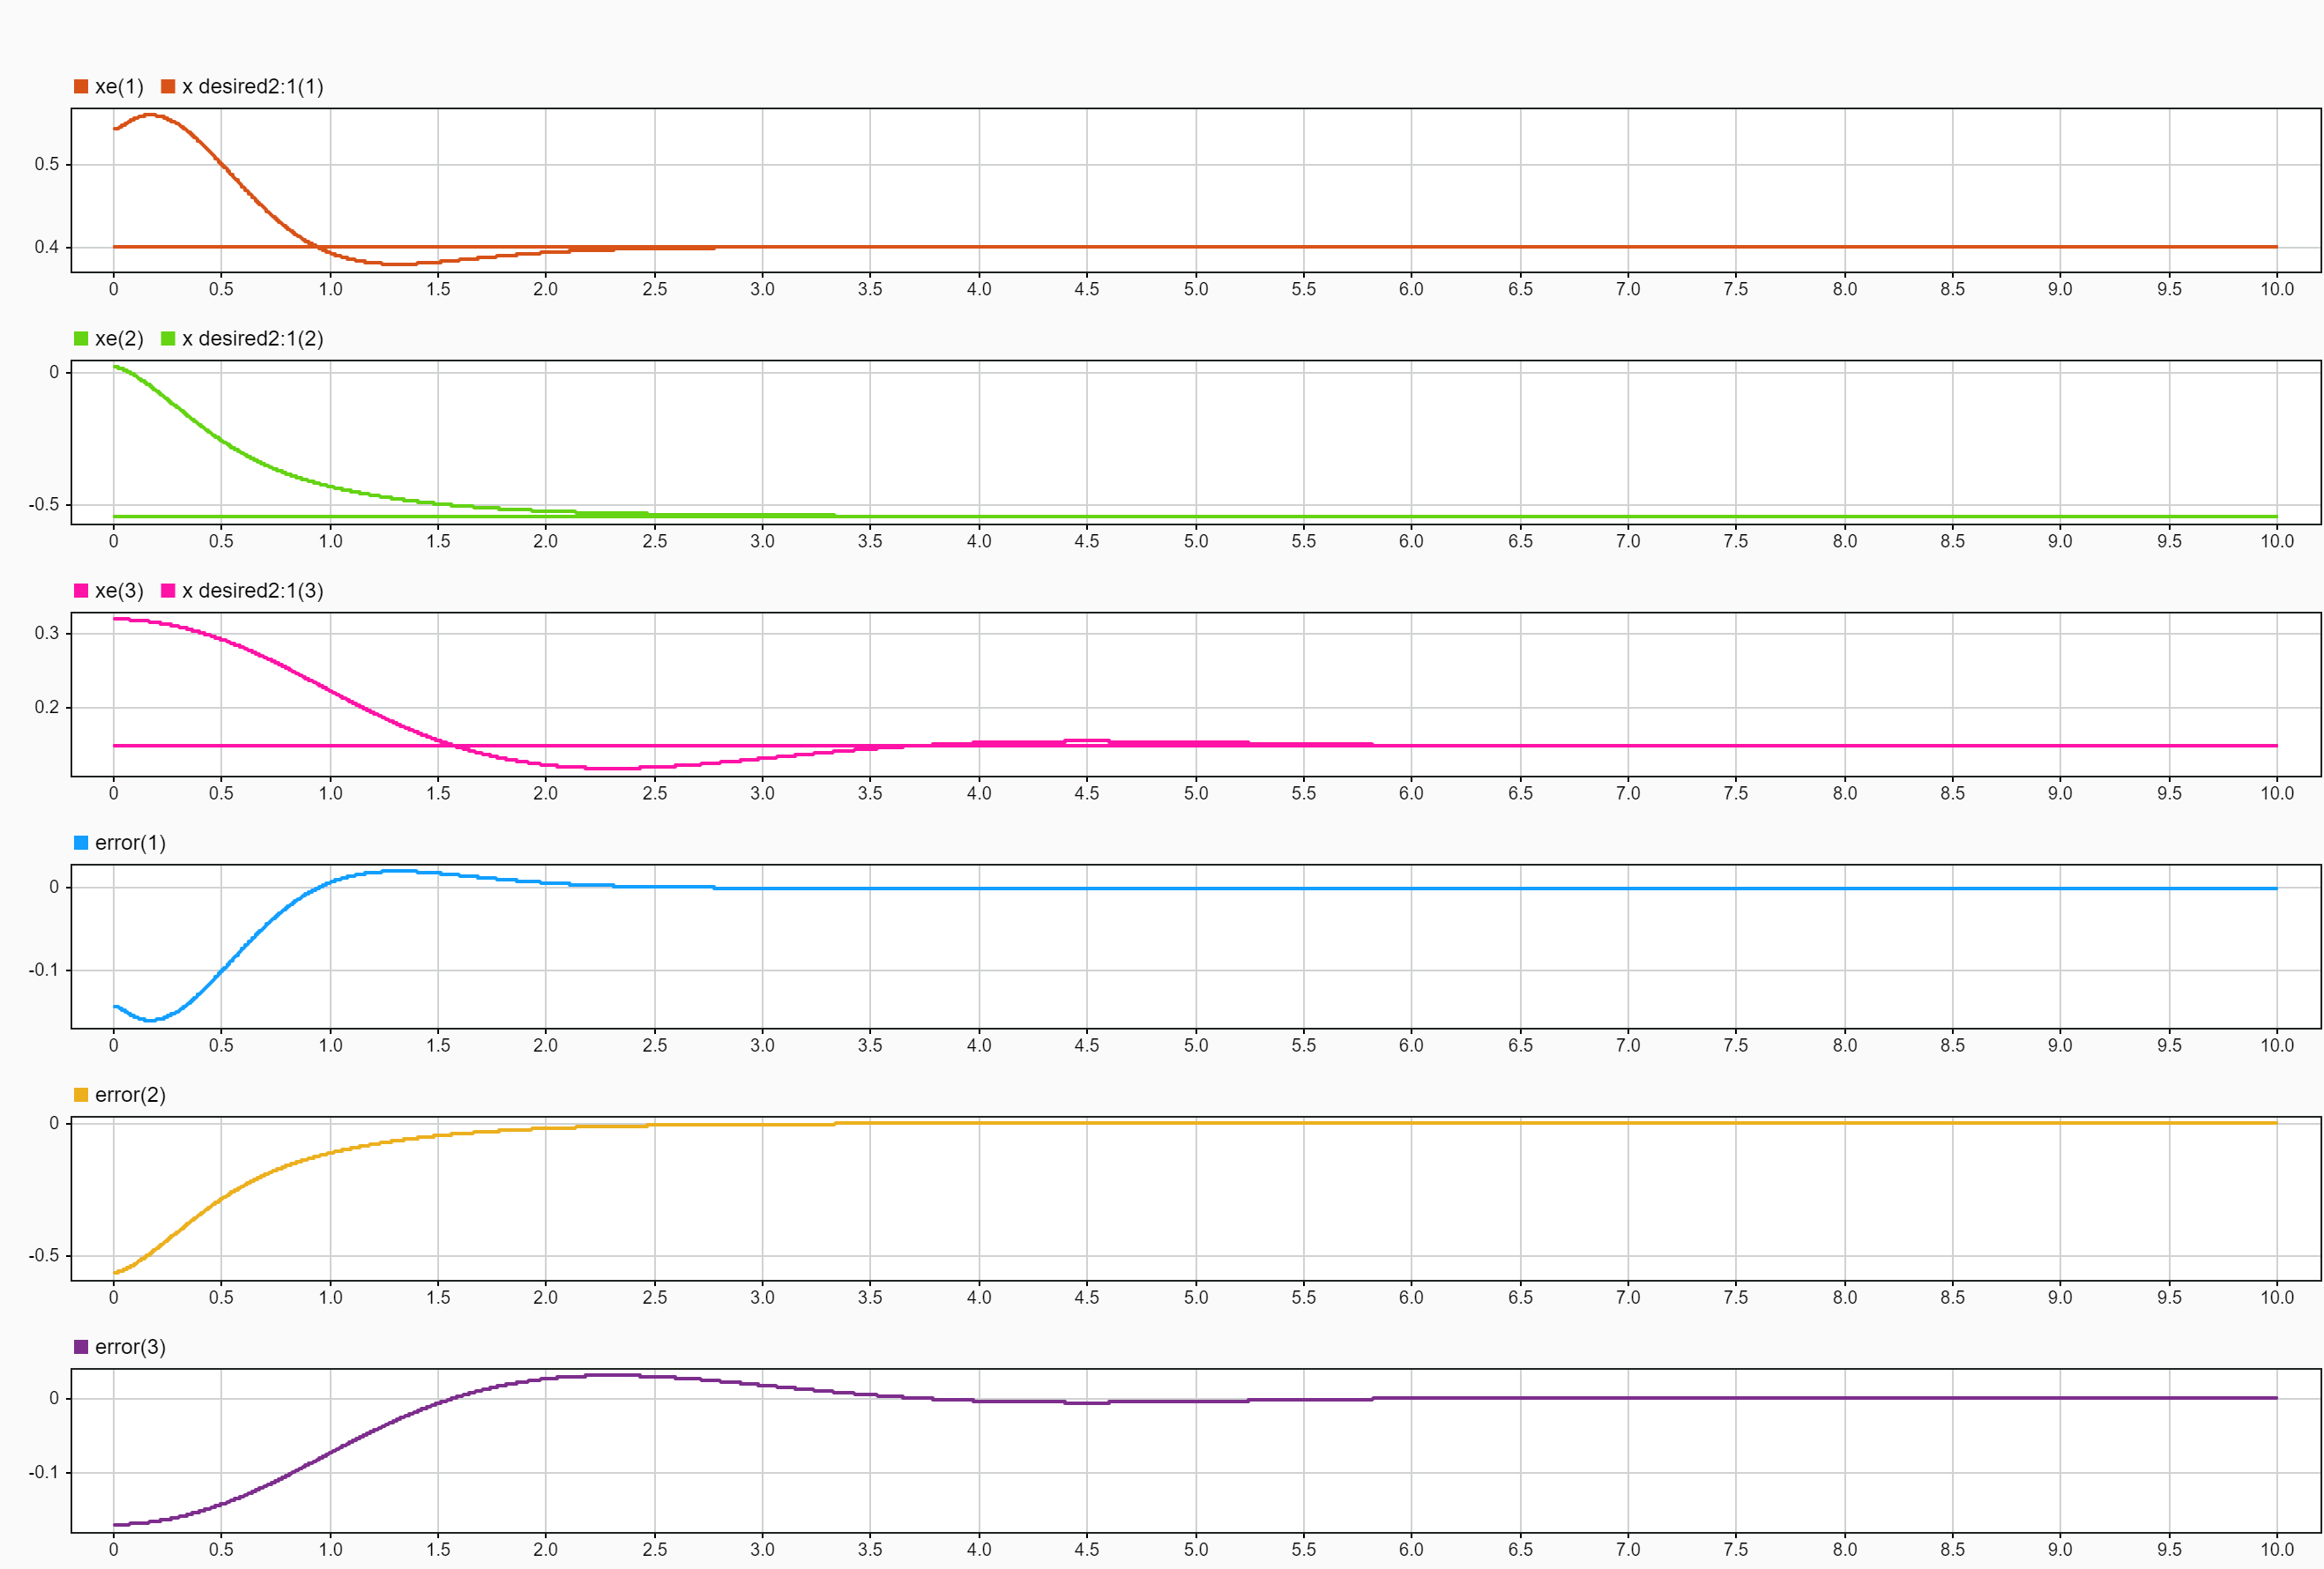
\includegraphics[width=1.4\textwidth]{../Simulink/Images/inverseDynamicOperationalSpaceReachablePosition.png}}
    \caption{The robot can reach the position and the rror goes to zero}
    \label{fig:The robot can reach the positionnn}
\end{figure}


\newpage



In the second one we have:

\begin{figure}[H]
    \centering
    \makebox[\textwidth][c]{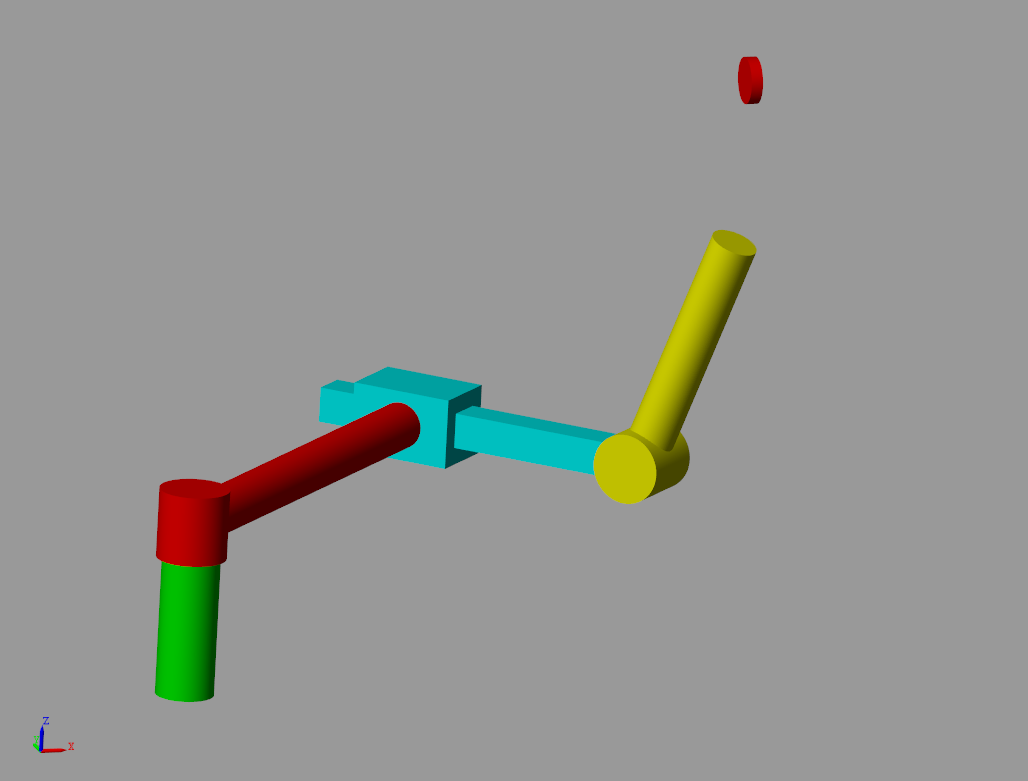
\includegraphics[width=0.4\textwidth]{../Simulink/Images/inverseDynamic.png}}
    \caption{The robot can't reach the position}
    \label{fig:The robot can't reach the position}
\end{figure}

\begin{figure}[H]
    \centering
    \makebox[\textwidth][c]{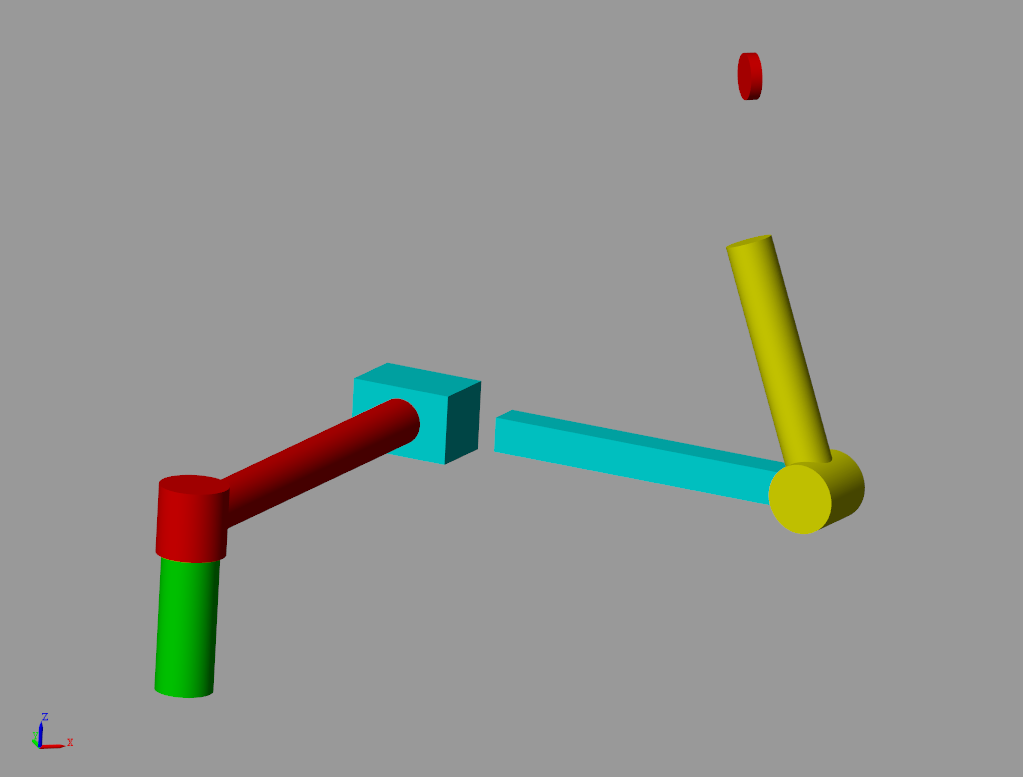
\includegraphics[width=0.4\textwidth]{../Simulink/Images/inverseDynamic1.png}}
    \caption{The robot can't reach the position}
    \label{fig:The robot can't reach the positionn}
\end{figure}

where we can note that the robot if can't reach the position, it will obscillate but it does not reach the zero steady state error.



\begin{figure}[H]
    \centering
    \makebox[\textwidth][c]{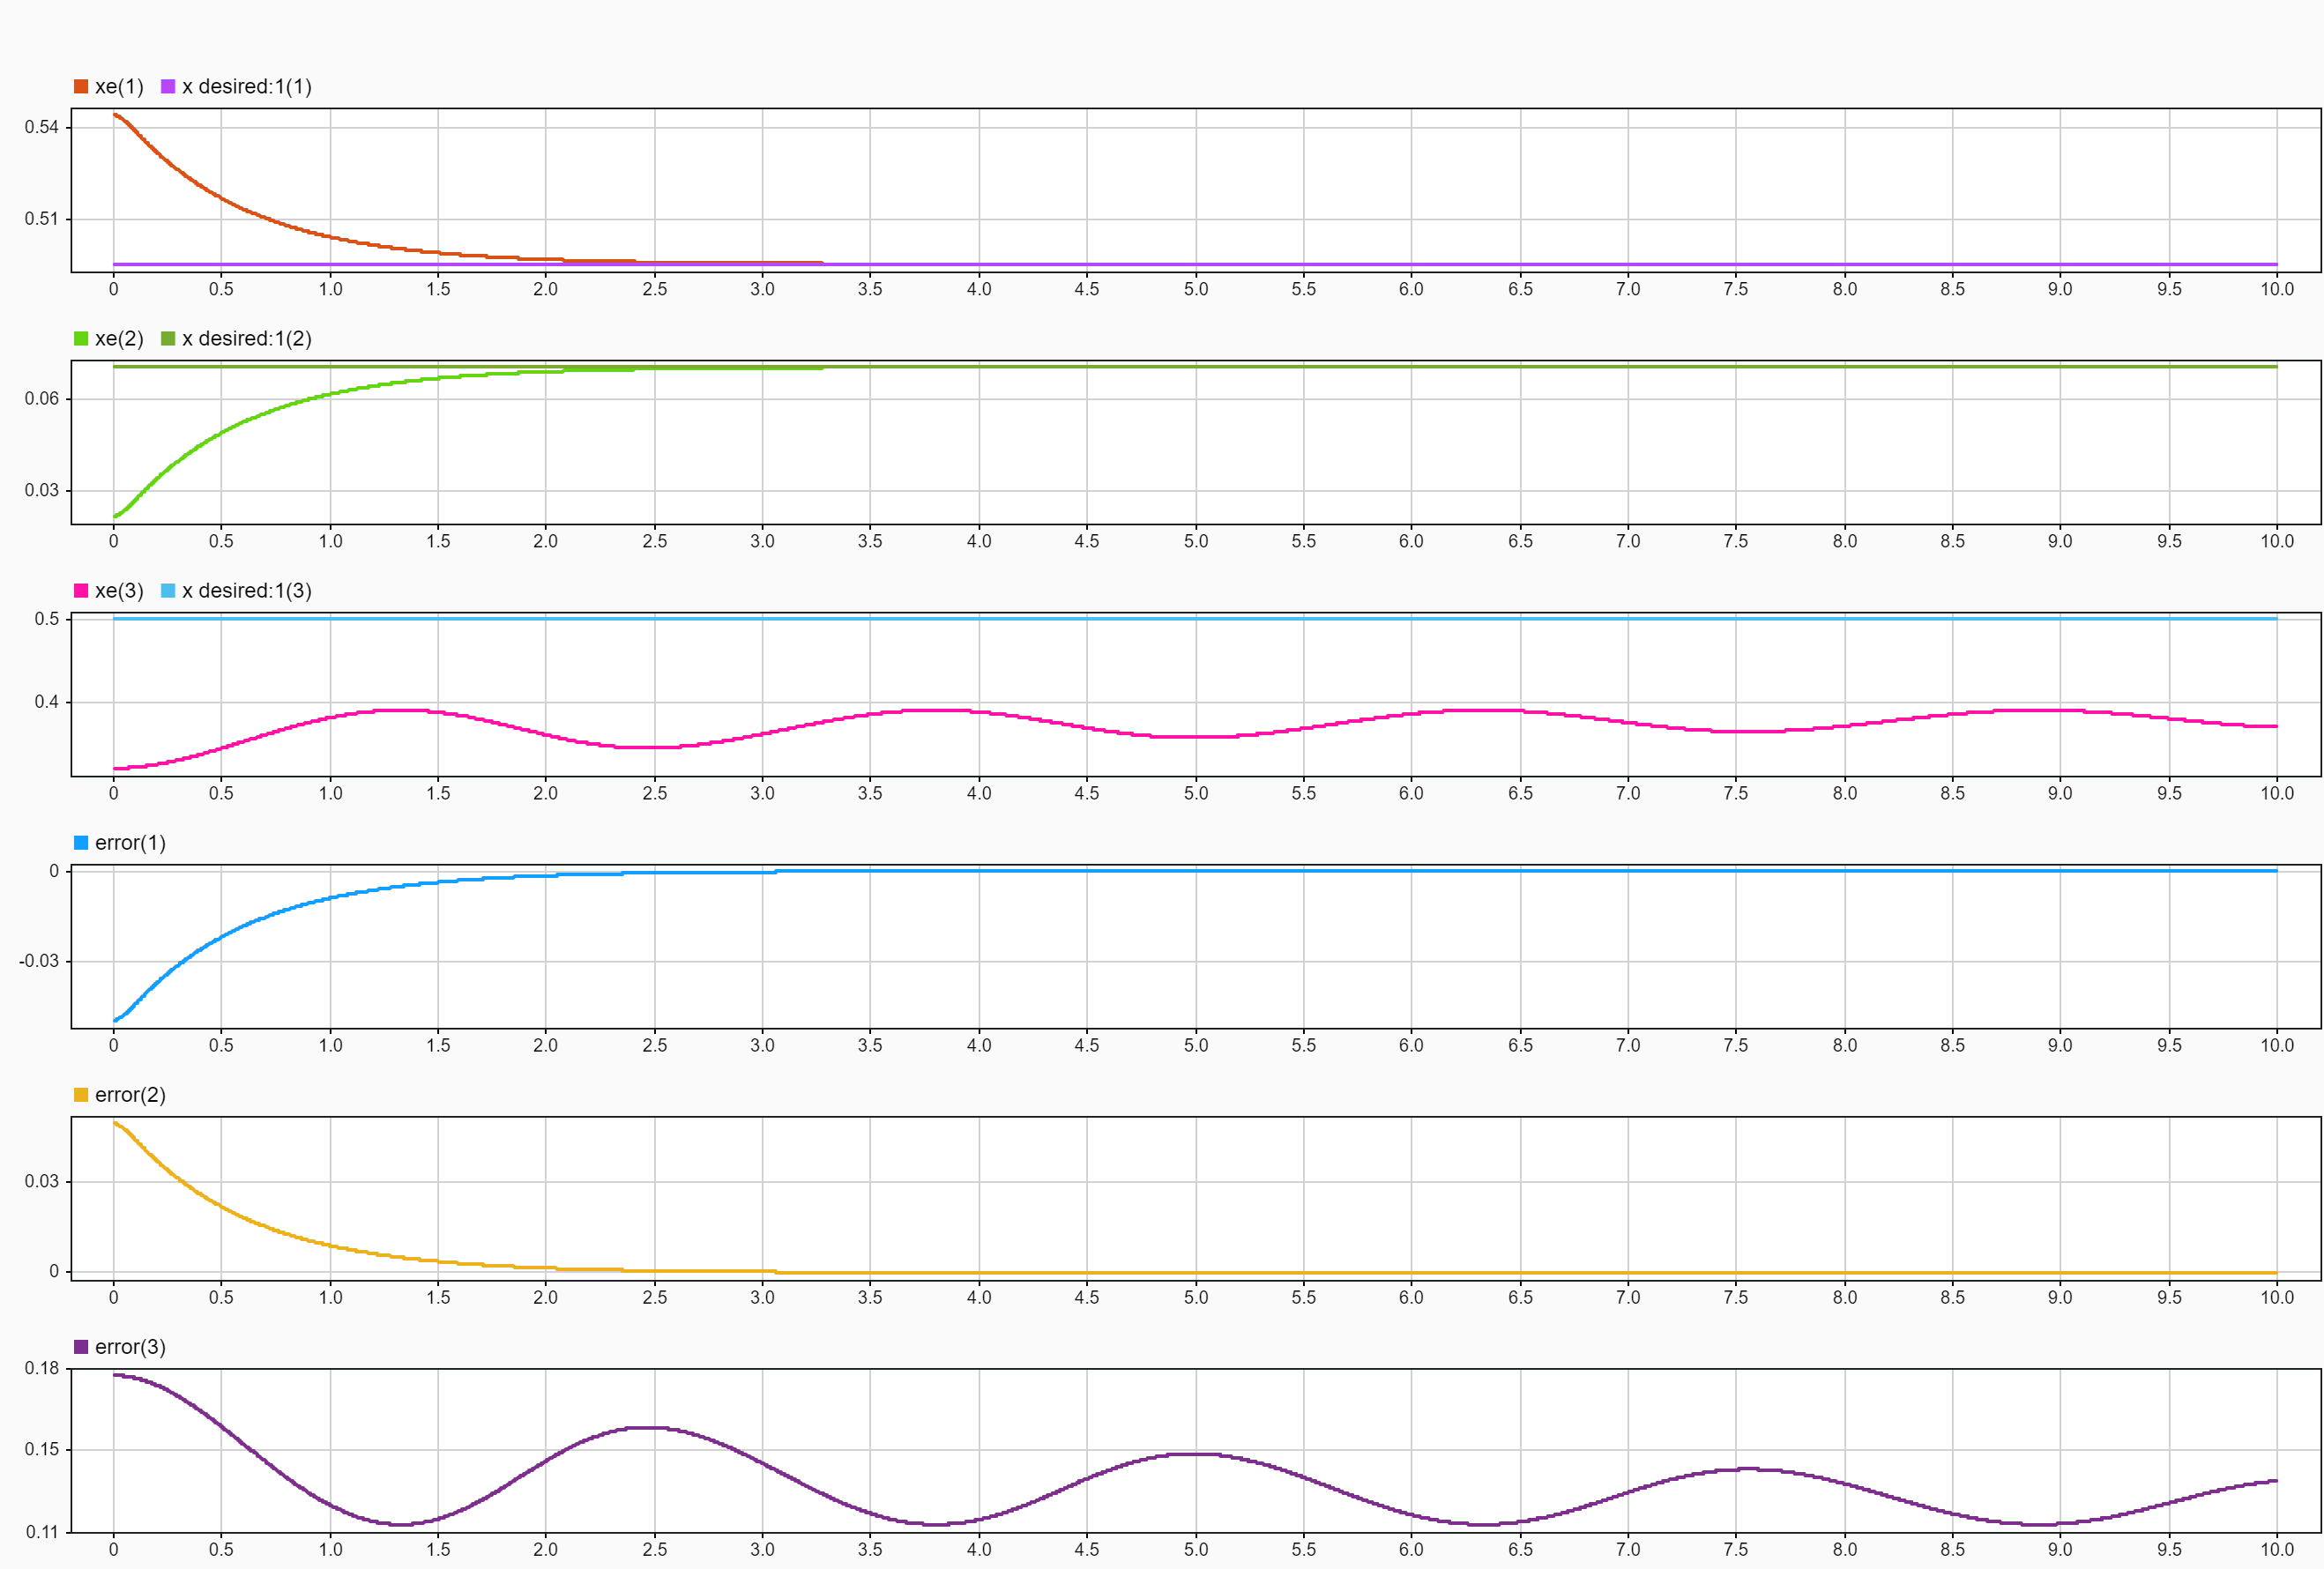
\includegraphics[width=1.6\textwidth]{../Simulink/Images/inverseDynamicOperationalSpaceNONreachablePosition.png}}
    \caption{The robot can't reach the position and the error NOT goes to zero}
    \label{fig:The robot can't reach the positionnm}
\end{figure}










\newpage

\subsection{Compliance control}

In this control scheme we modify the PD with gravity compensation control scheme.

Also in the compliance control we have 2 distinct cases. The first on is the passive compliance control, where the wall acts like a spring.
Off course the robot in both cases will not reach the desired position, due to the wall that is pushing it back.

\begin{figure}[H]
    \centering
    \makebox[\textwidth][c]{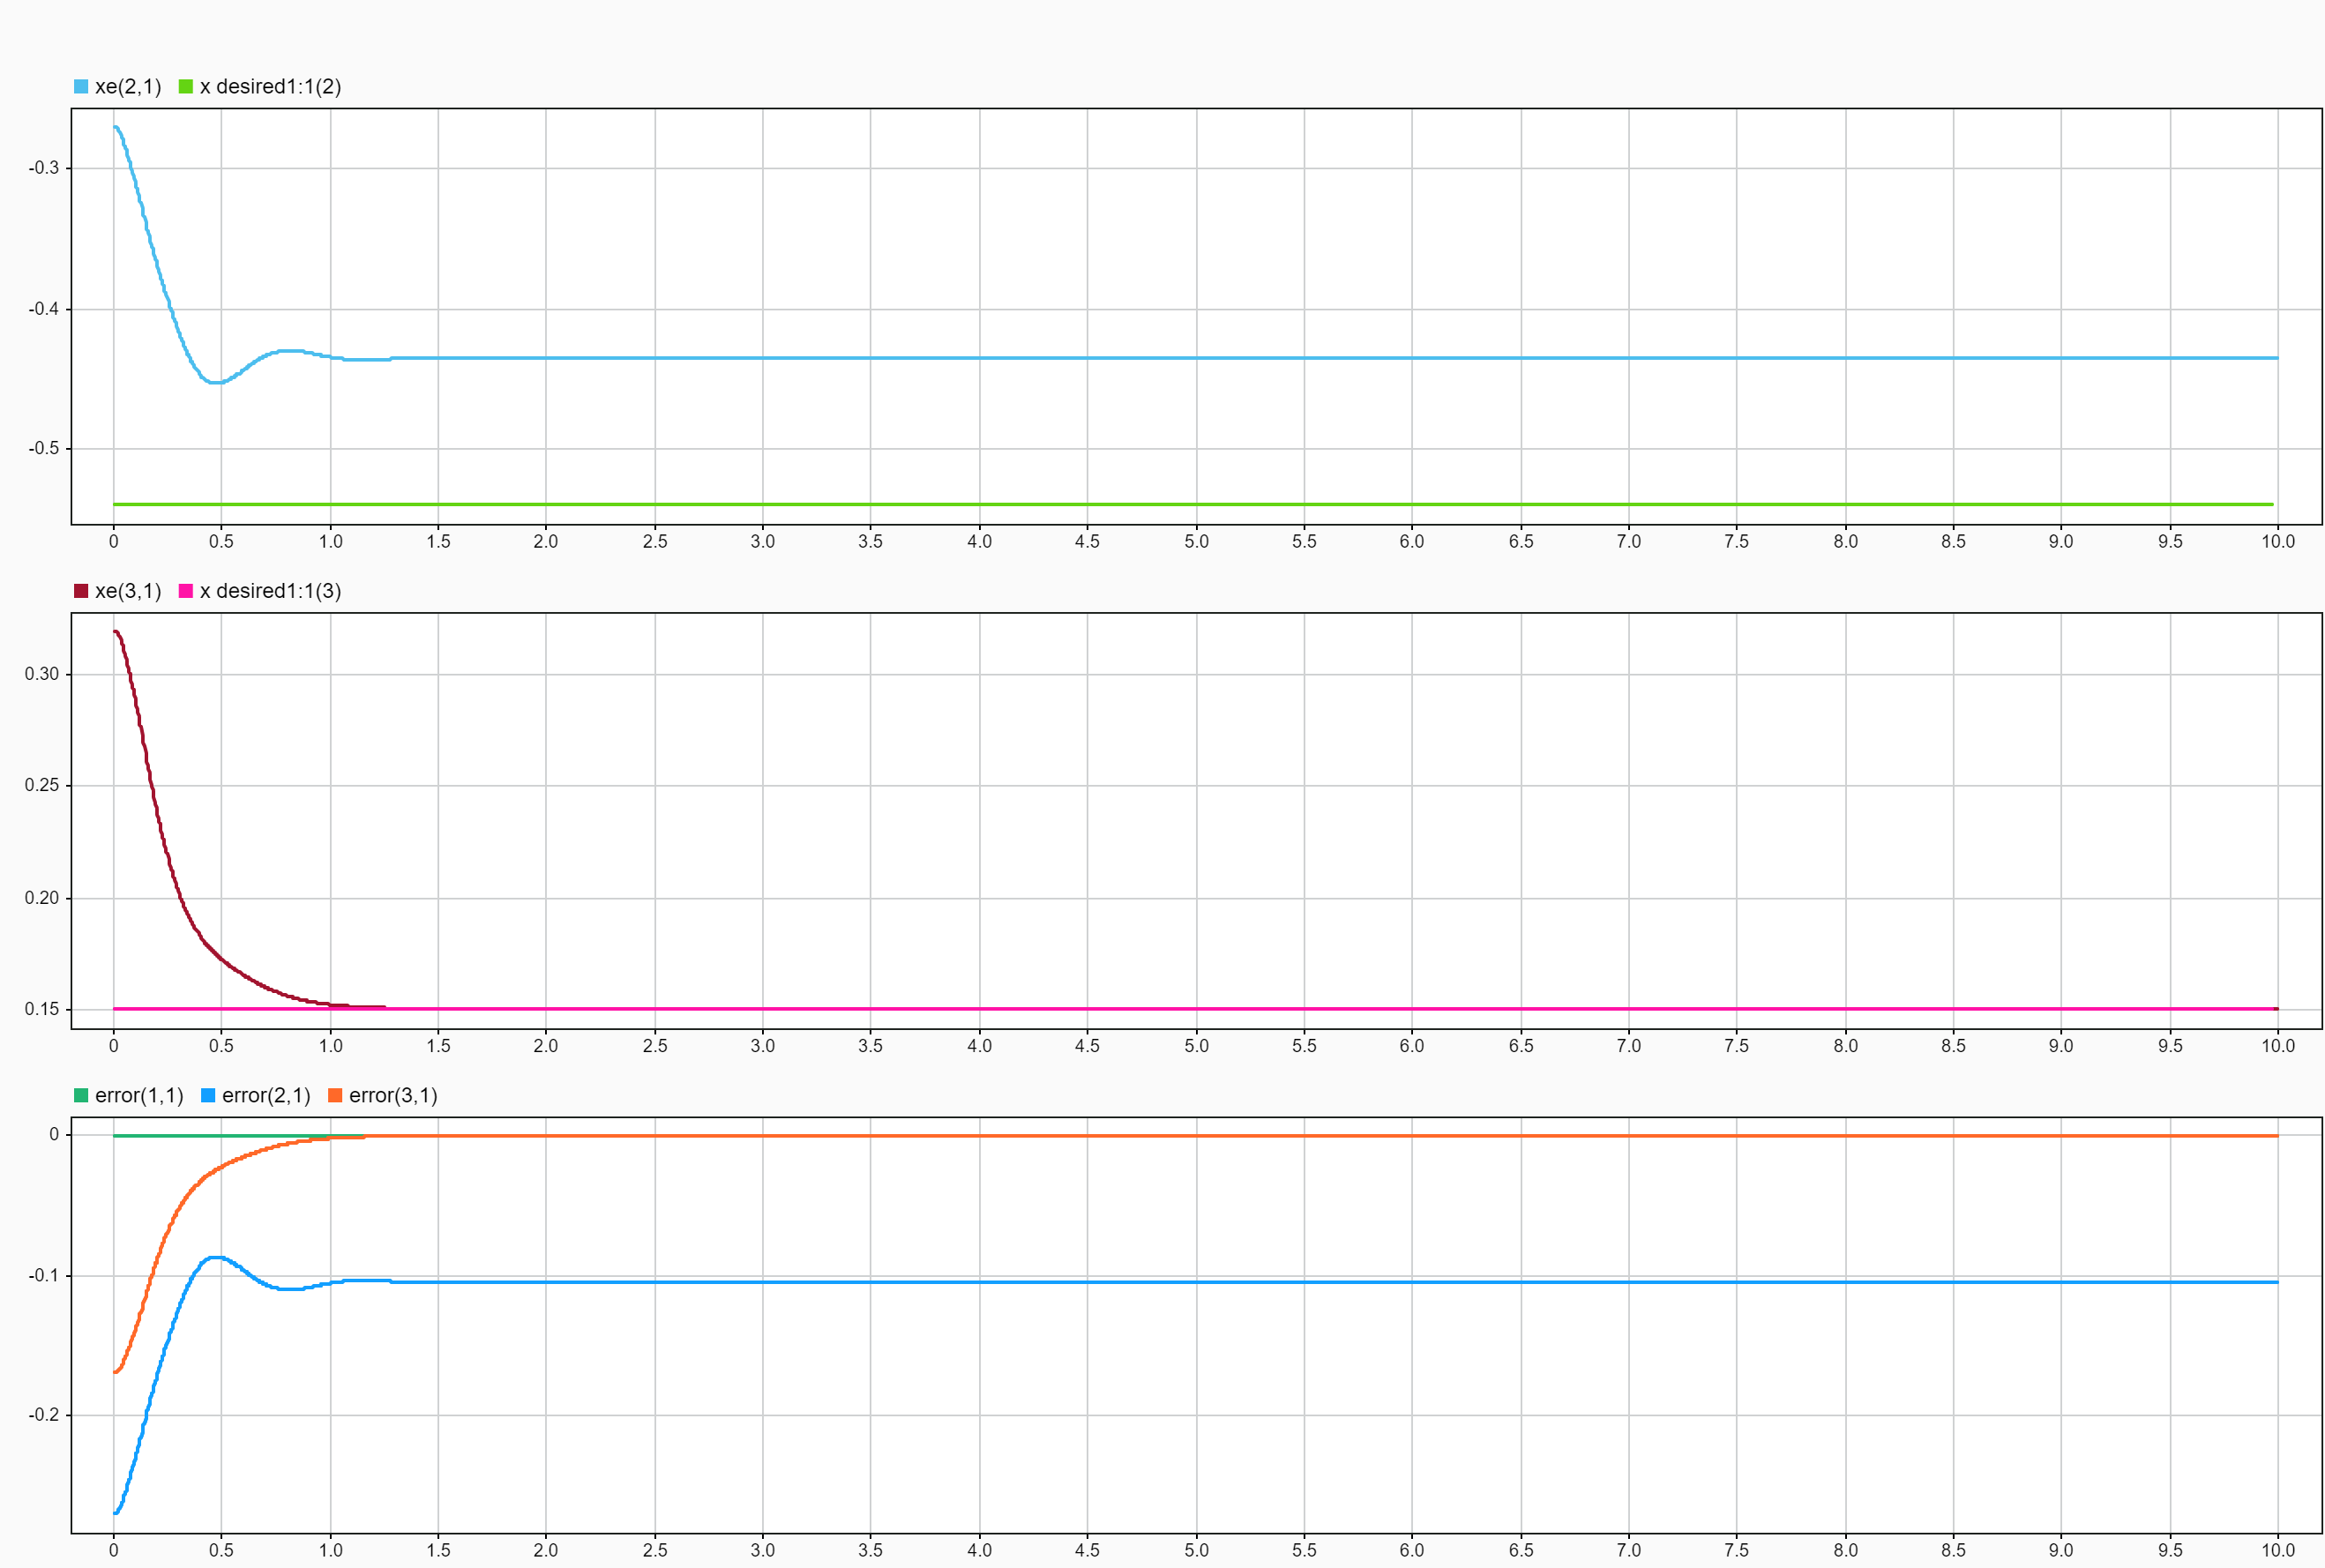
\includegraphics[width=1.6\textwidth]{../Simulink/Images/passiveCompliance.png}}
    \caption{passiveCompliance}
    \label{fig:passiveCompliance}
\end{figure}








in the second case, that is very different from the first one, we have an active compliace control, where, with an s-function, we compute dinamicly the error between the desired position and the actual one, and we use this error to compute the torques to be imparted to the motors.

In particular we use this particular Jacobian, derivative from this formula:

\begin{equation}
    \dot{\tilde{x}} = -T_A^{-1}(\phi_{d,e}) \begin{bmatrix} R_d^T & O \\ O & R_d^T \end{bmatrix} J(q) \dot{q} = -J_{Ad}(q, \tilde{x}) \dot{q}
\end{equation}

In super important to understand that the T matrix, is the transformation matrix from the end effector to the desired position, as reported in the matlab code below:

\begin{lstlisting}[style=Matlab-editor]
Td = [eye(3), desired_position; 
      0 0 0 1];

% end effector frame
Te = A_b_ee;

% desired position in the end effector frame
T_D_e = [Td(1:3, 1:3)' * Te(1:3, 1:3), Td(1:3, 1:3)' * (Te(1:3, 4) - Td(1:3, 4));
            0 0 0 1];

phi = atan2(T_D_e(2, 3), T_D_e(1, 3));
gamma = acos(T_D_e(3, 3));
% psi = atan2(A_b_ee(3, 2), -A_b_ee(3, 1));

T_zyz = [0, -sin(phi), cos(phi) * sin(gamma);
            0, cos(phi), sin(phi) * sin(gamma);
            1, 0, cos(gamma)];

Ta = blkdiag(eye(3), T_zyz);

Jad = inv(Ta) * blkdiag(Td(1:3, 1:3)', Td(1:3, 1:3)') * J_analytical;

block.OutputPort(1).Data = Jad(1:3, 1:3);



\end{lstlisting}



\begin{figure}[H]
    \centering
    \makebox[\textwidth][c]{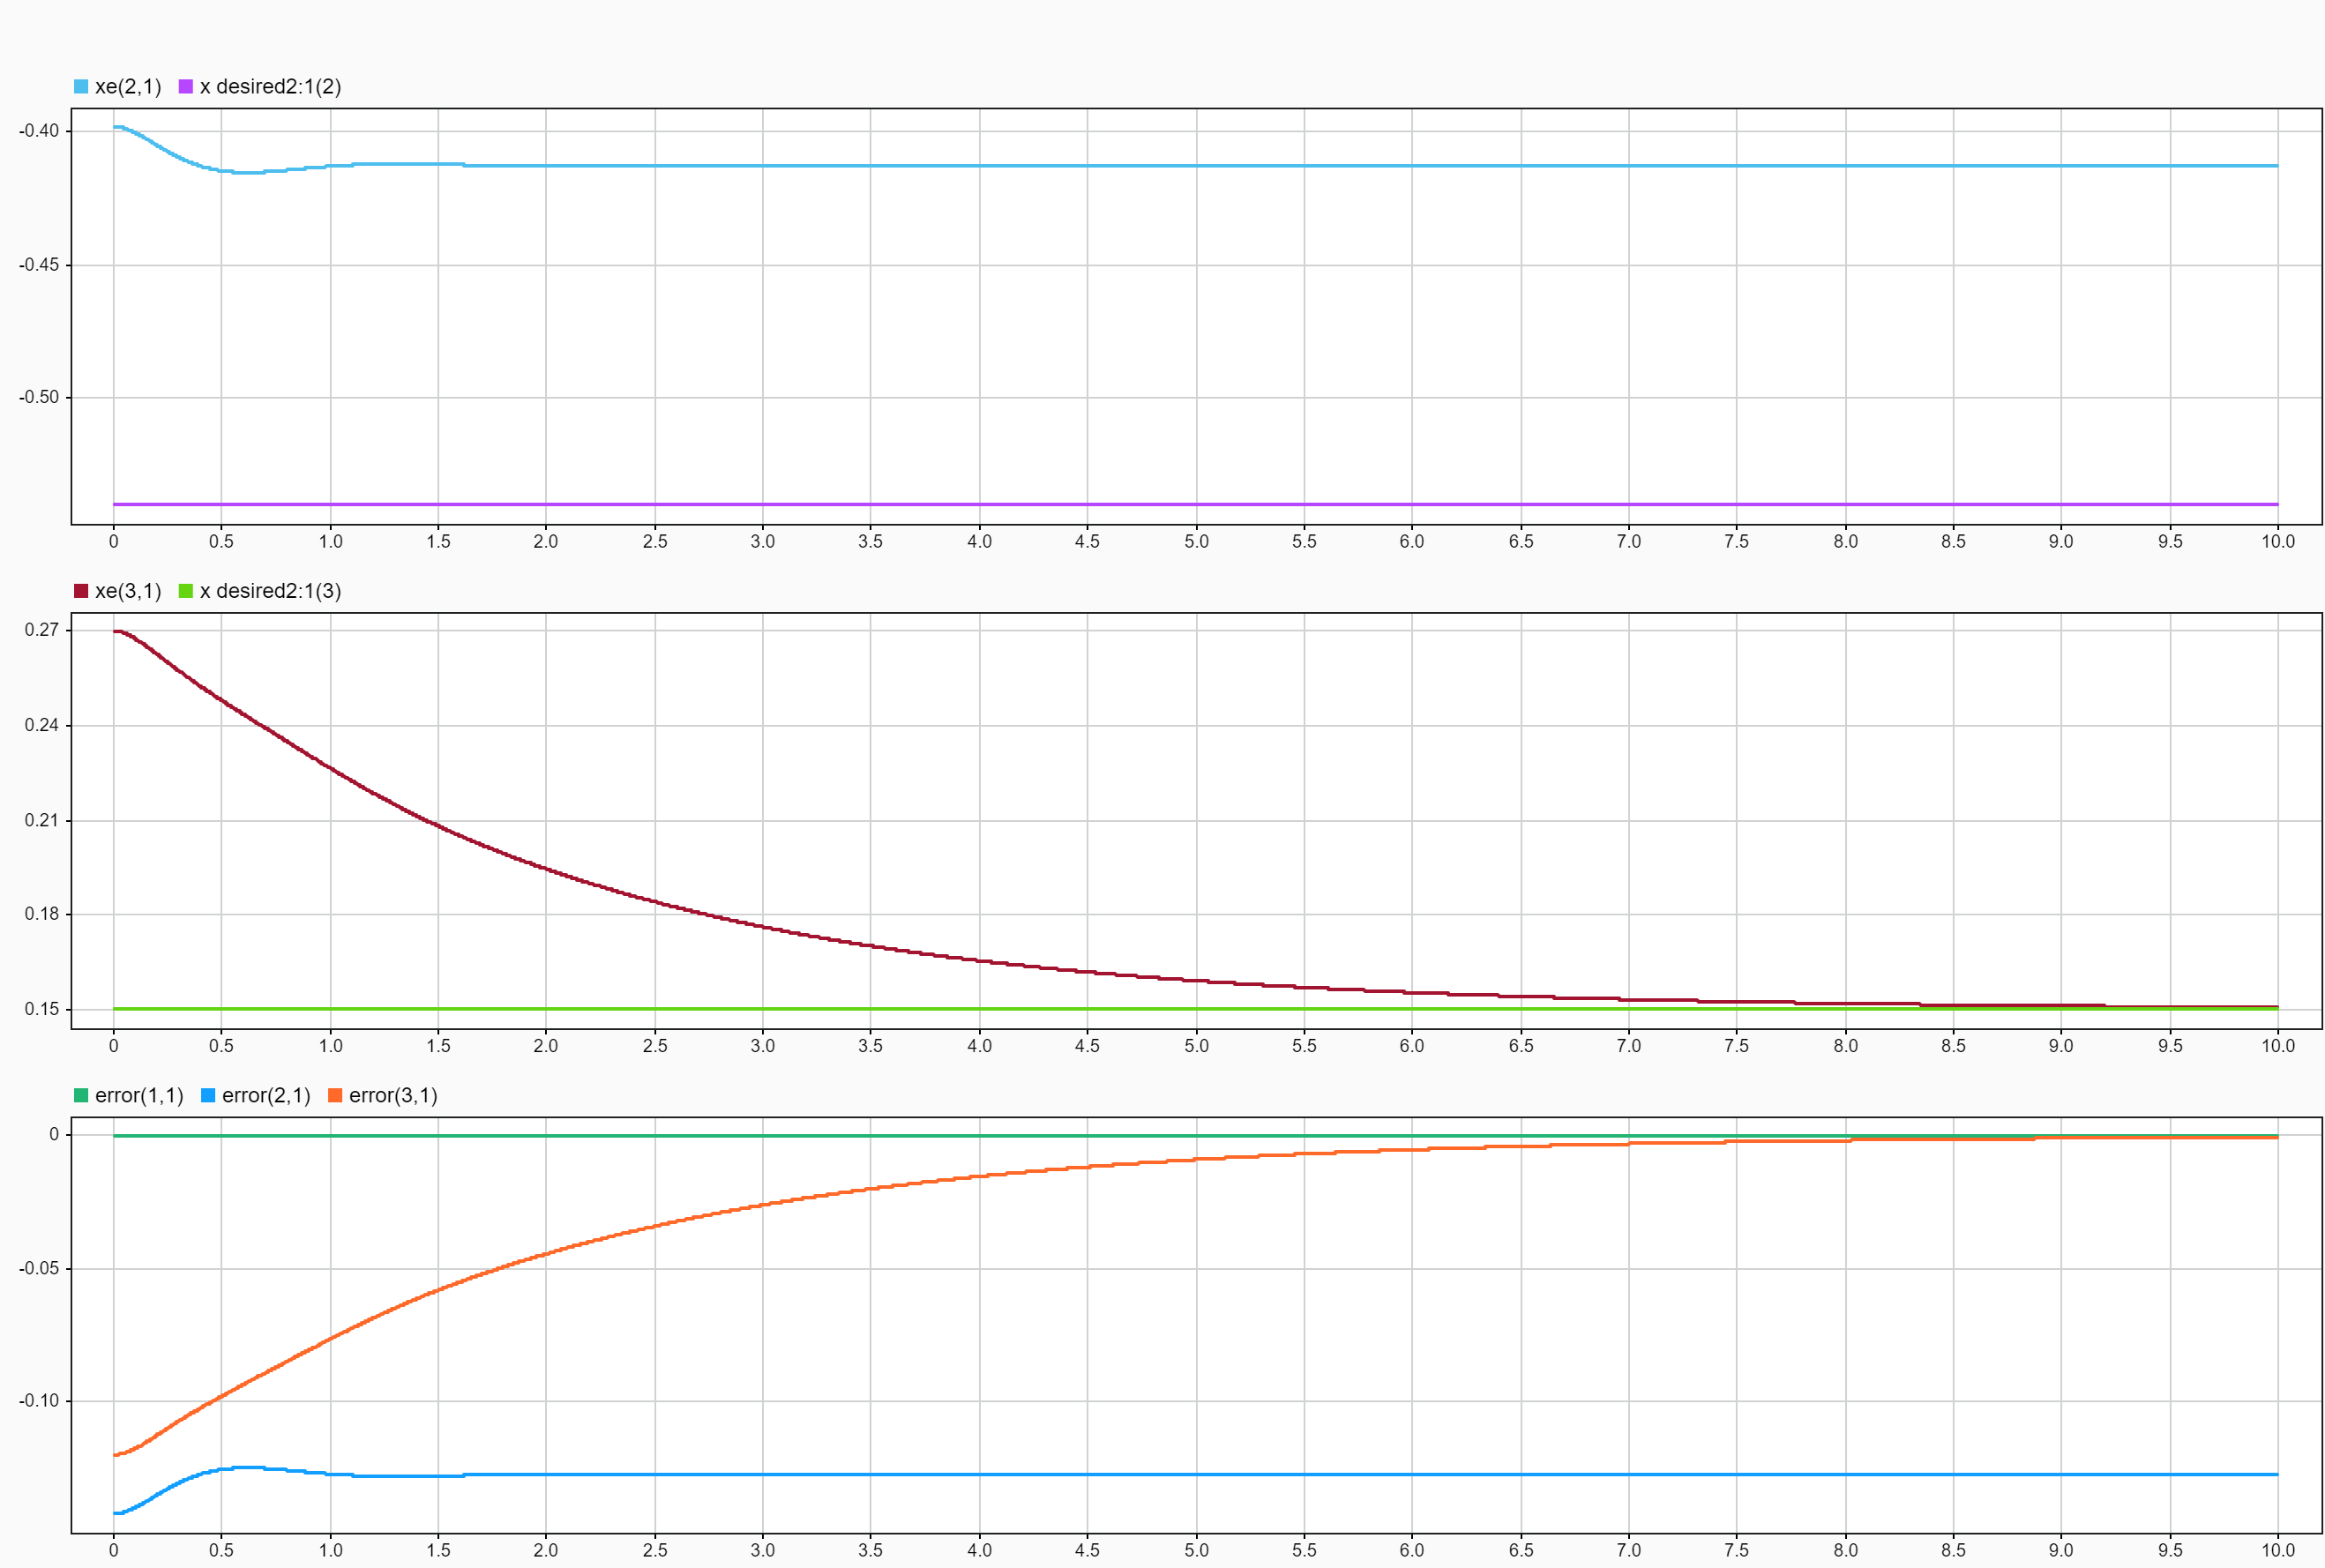
\includegraphics[width=1.6\textwidth]{../Simulink/Images/activeCompliance.png}}
    \caption{activeCompliance}
    \label{fig:activeCompliance}
\end{figure}

As expected we have an error on the second joint, where the "spring" of the wall is acting, and the robot is not able to reach the desired position.







\subsection{Force control}

\subsubsection{Block scheme of force control with inner position loop}
\begin{figure}[H]
    \centering
    \makebox[\textwidth][c]{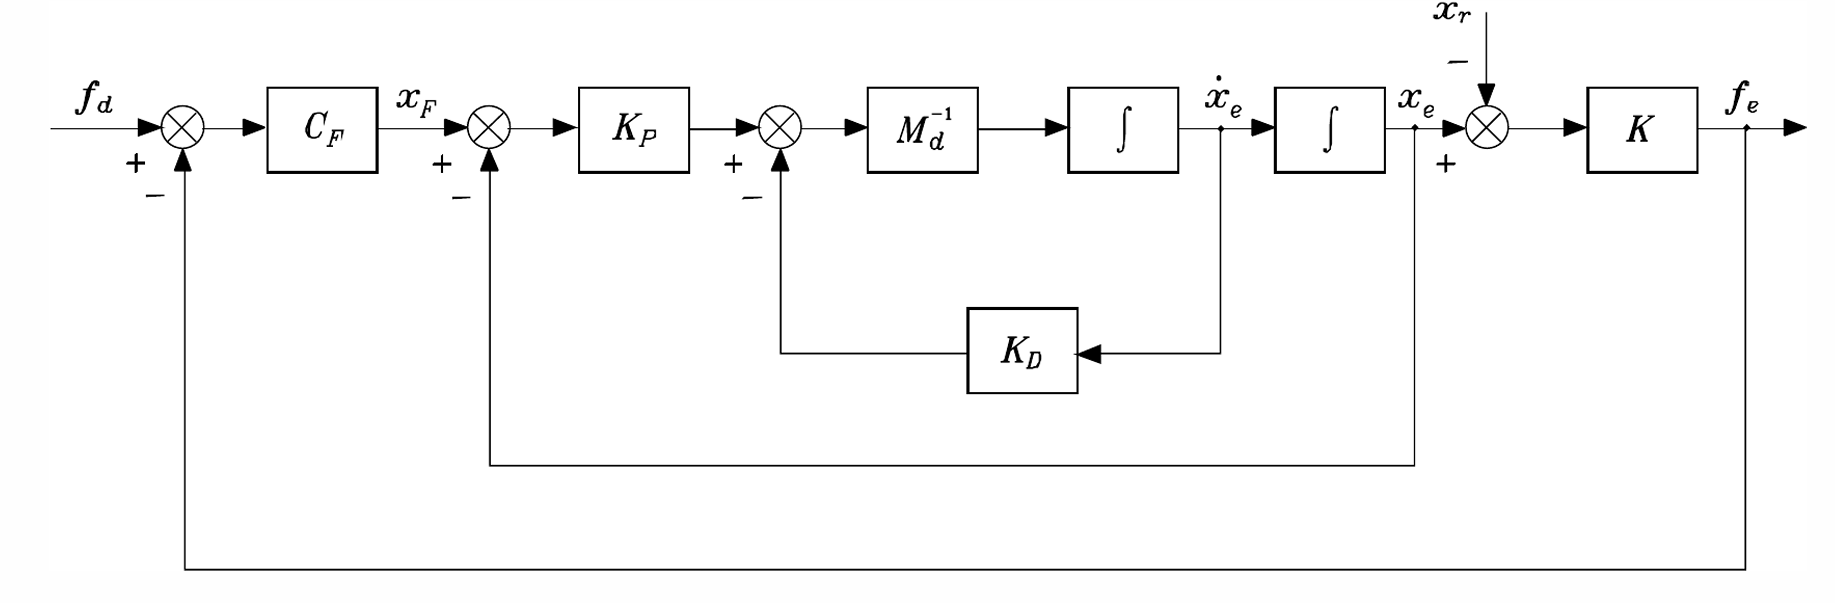
\includegraphics[width=1\textwidth]{../Simulink/Images/force_control_inner_position.png}}
    \caption{Block scheme of force control with inner position loop.}
    \label{fig:Block scheme of force control with inner position loop.}
\end{figure}


\begin{figure}[H]
    \centering
    \makebox[\textwidth][c]{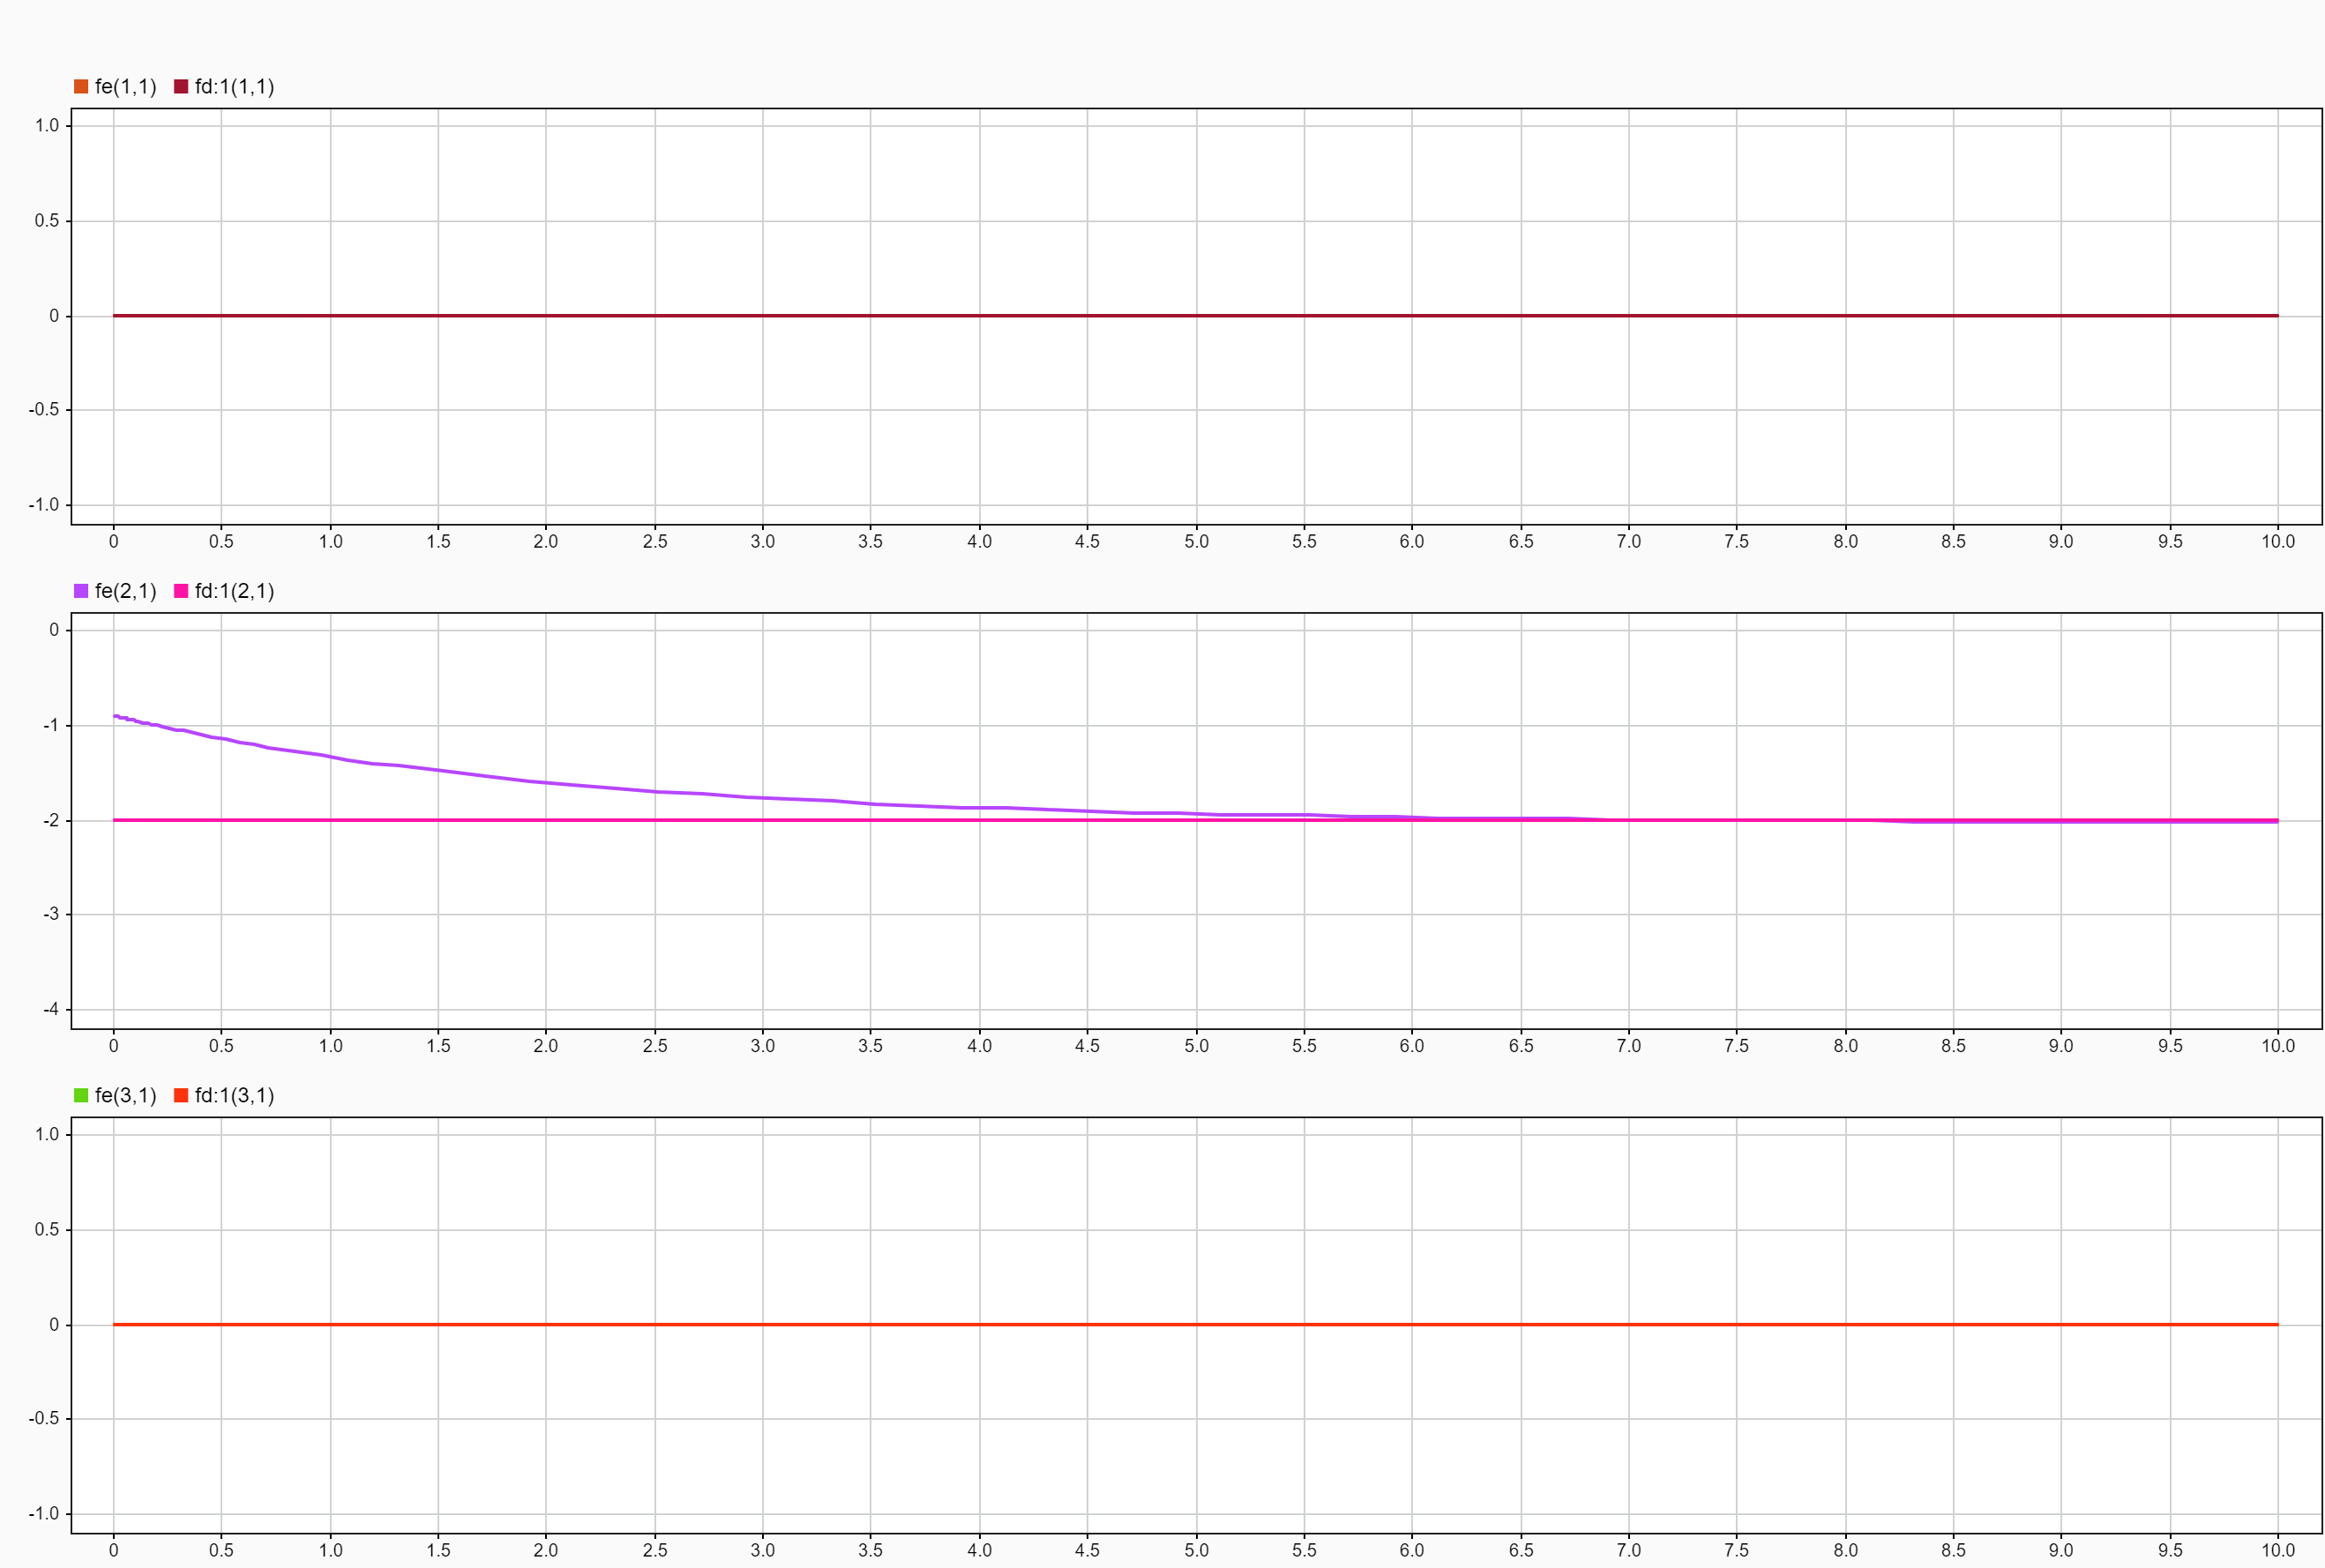
\includegraphics[width=1.2\textwidth]{../Simulink/Images/force_control_inner_position_graph.png}}
    \caption{force control inner position}
    \label{fig:force_control_inner_position_graph}
\end{figure}


In the control scheme, if we assume Cf as a constant matrix we cannot reach the zero steady state error.
But if we use an integrator, we will have the zero error.

\begin{equation}
    C_F(s) = K_F + K_i \frac{1}{s}
\end{equation}






\subsubsection{Block scheme of force control with inner velocity loop}
\begin{figure}[H]
    \centering
    \makebox[\textwidth][c]{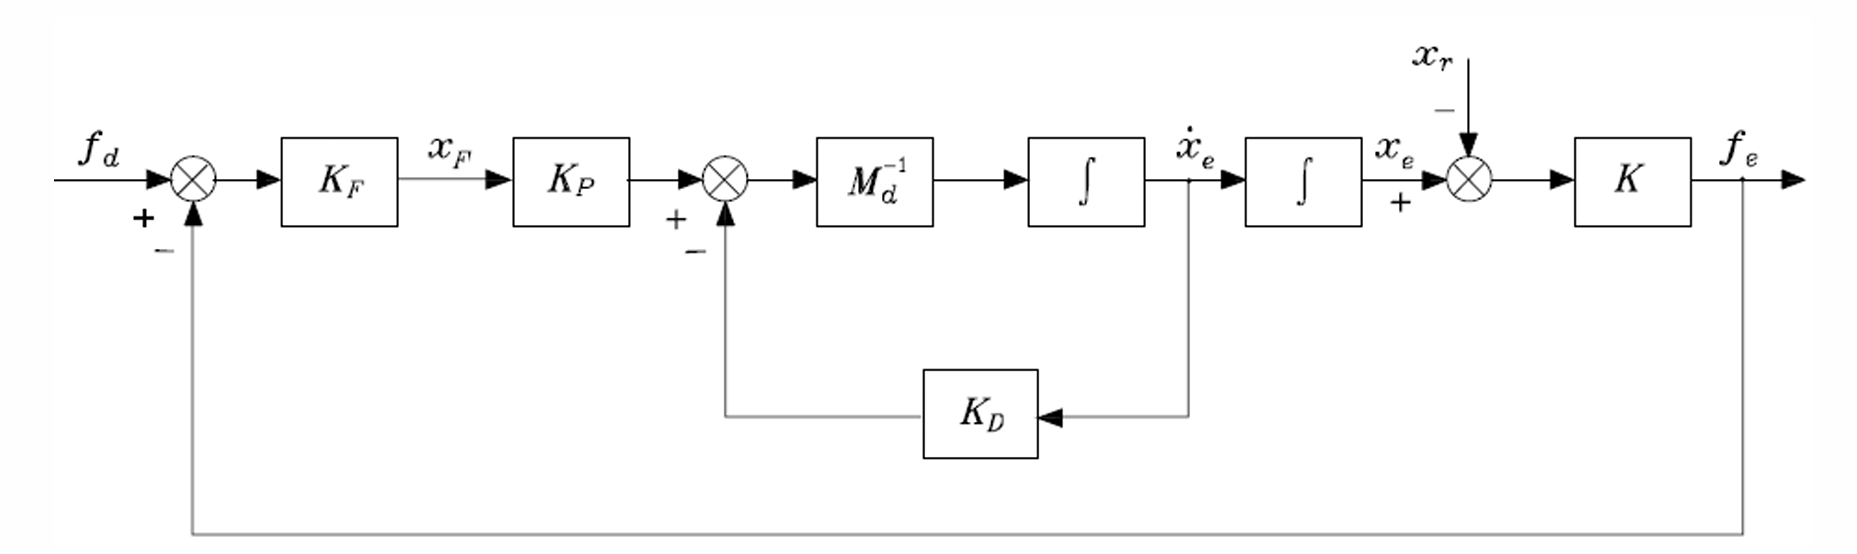
\includegraphics[width=1\textwidth]{../Simulink/Images/velocity_loop.png}}
    \caption{Block scheme of force control with inner velocity loop.}
    \label{fig:Block scheme of force control with inner velocity loop.}
\end{figure}


\begin{figure}[H]
    \centering
    \makebox[\textwidth][c]{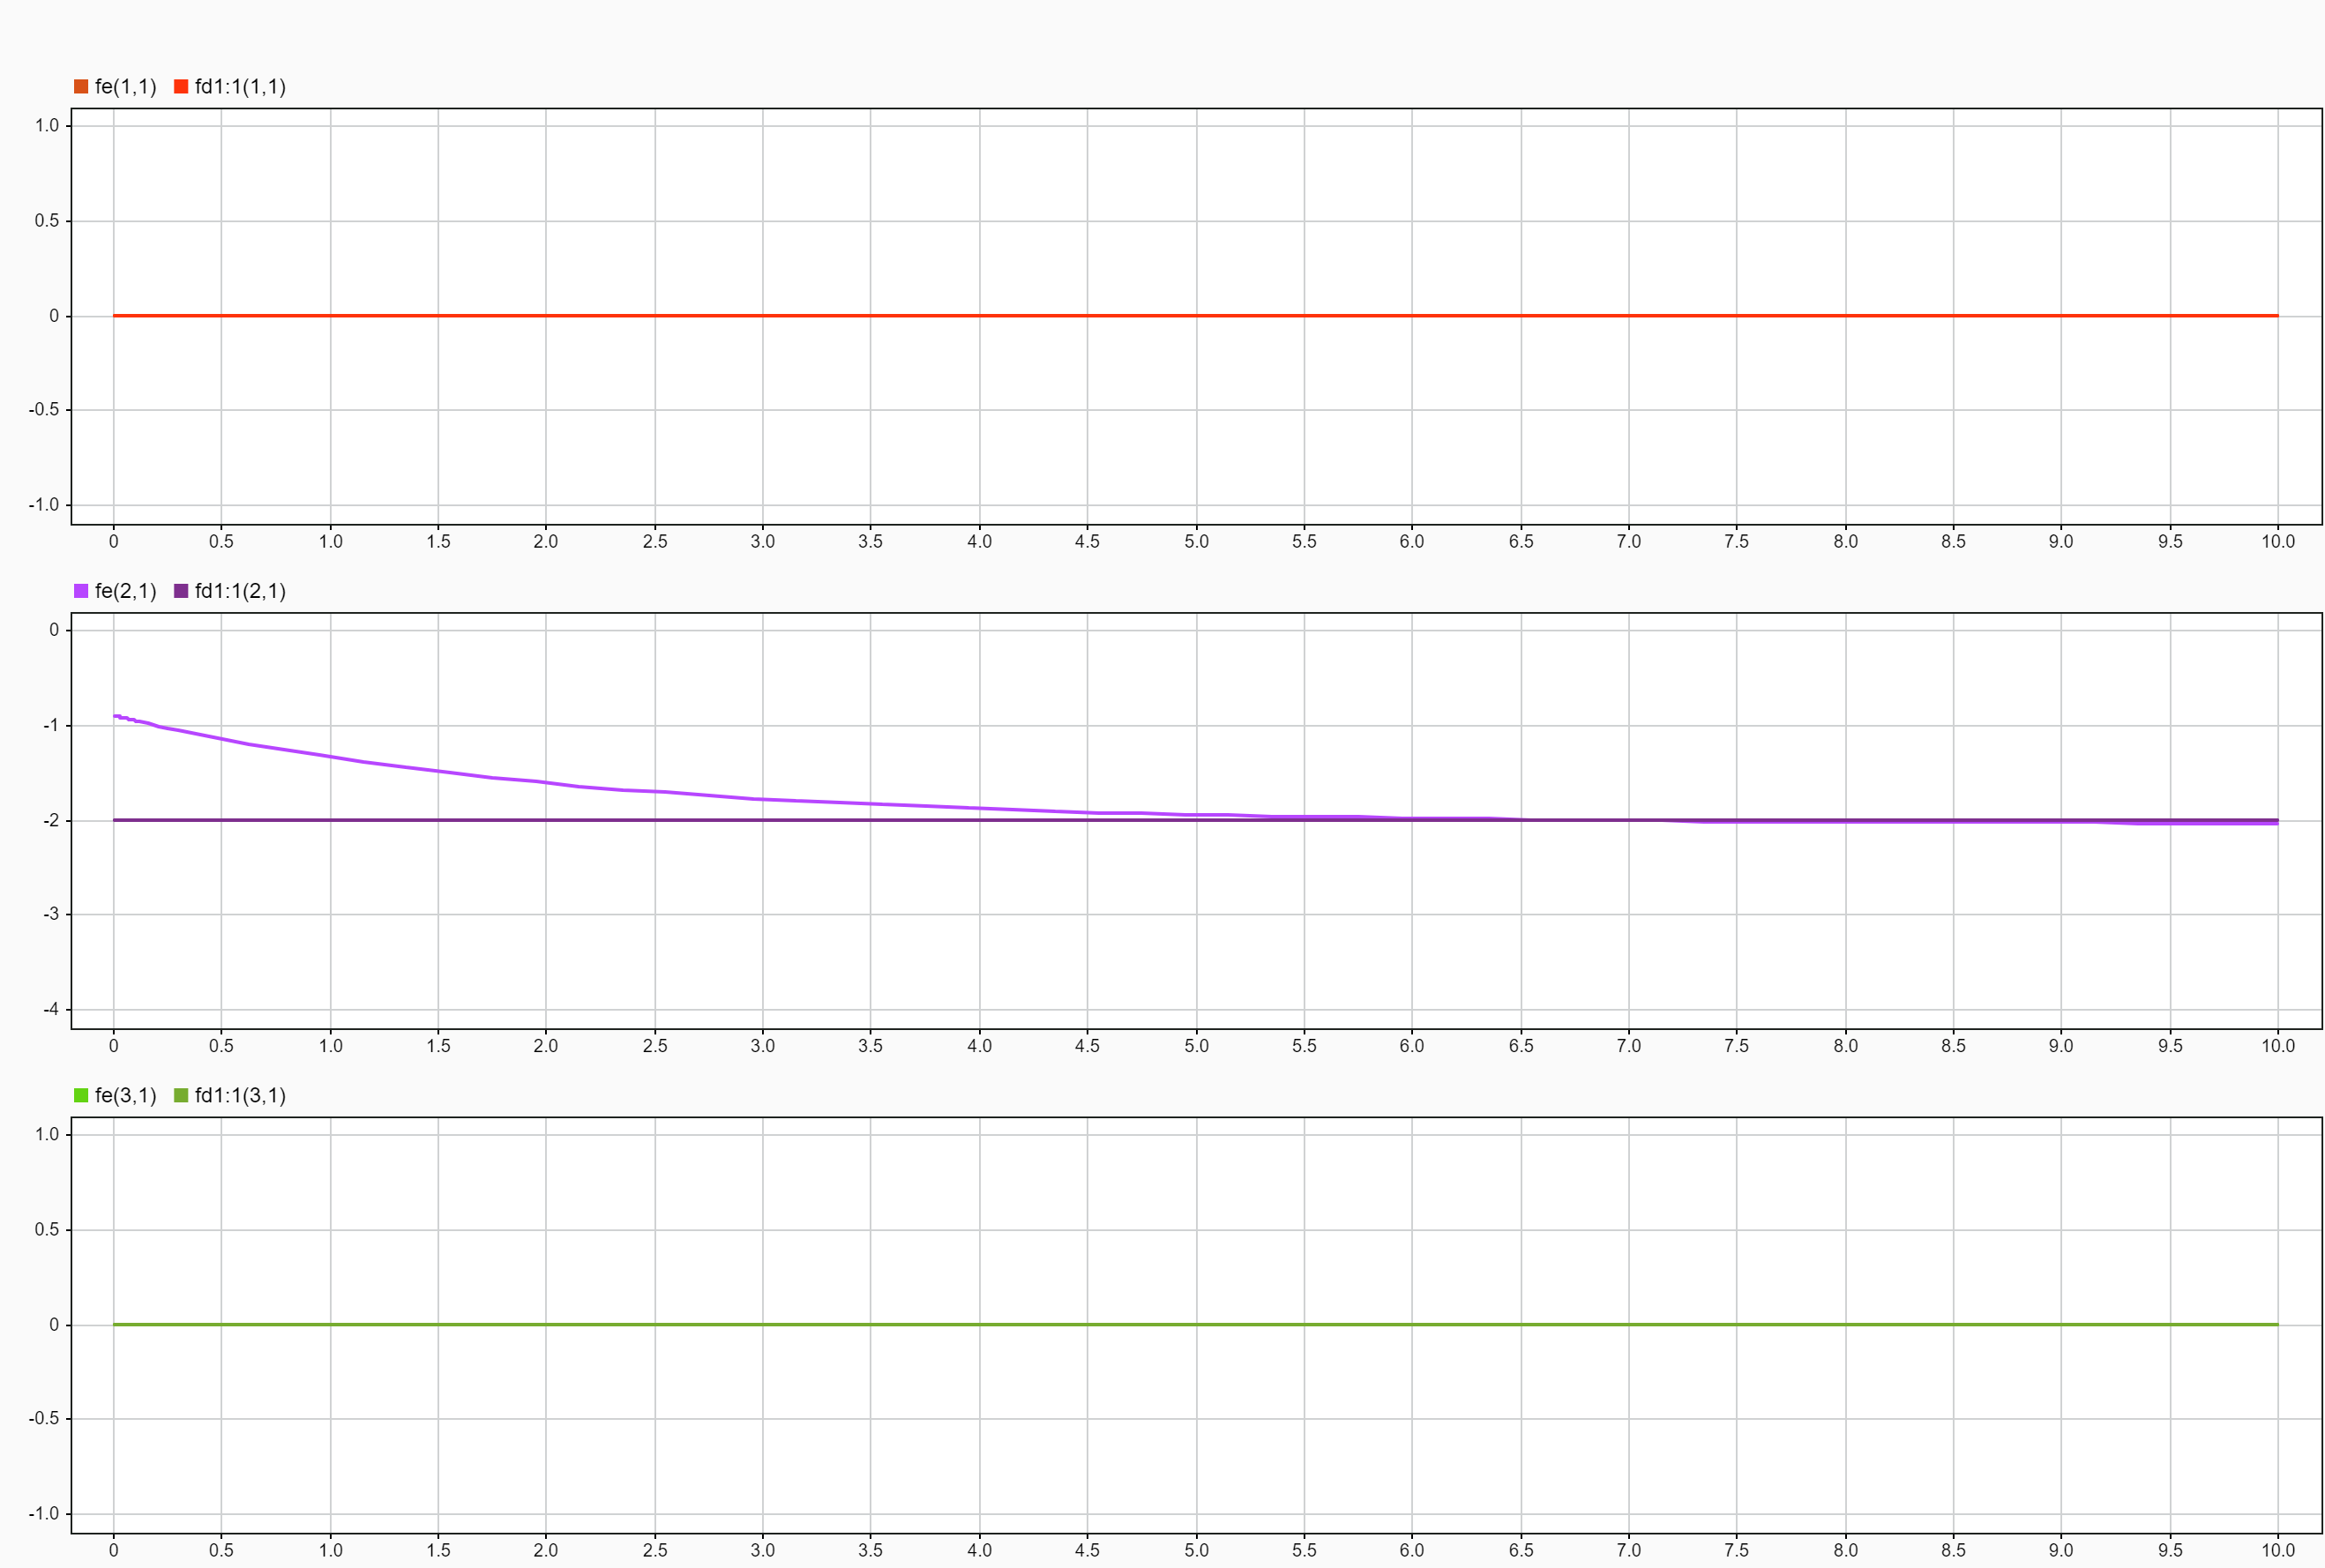
\includegraphics[width=1.2\textwidth]{../Simulink/Images/innerVelocityLoop.png}}
    \caption{force control inner velocity loop}
    \label{fig:force_control_inner_velocity_graph}
\end{figure}


\subsubsection{Block scheme of parallel force/position control}
\begin{figure}[H]
    \centering
    \makebox[\textwidth][c]{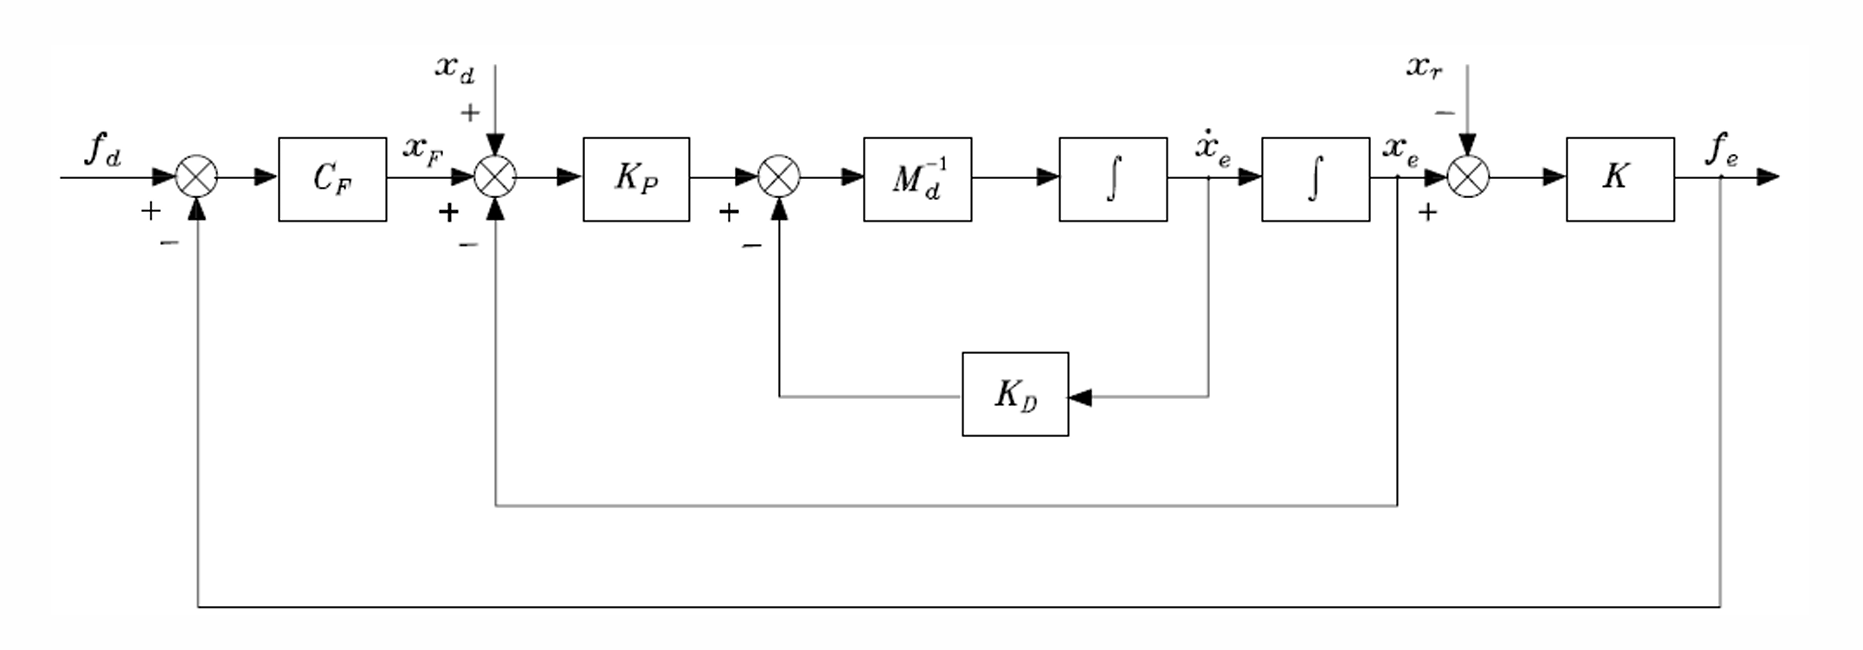
\includegraphics[width=1\textwidth]{../Simulink/Images/parallelForce.png}}
    \caption{Block scheme of parallel force/position control.}
    \label{fig:parallelForce}
\end{figure}


\begin{figure}[H]
    \centering
    \makebox[\textwidth][c]{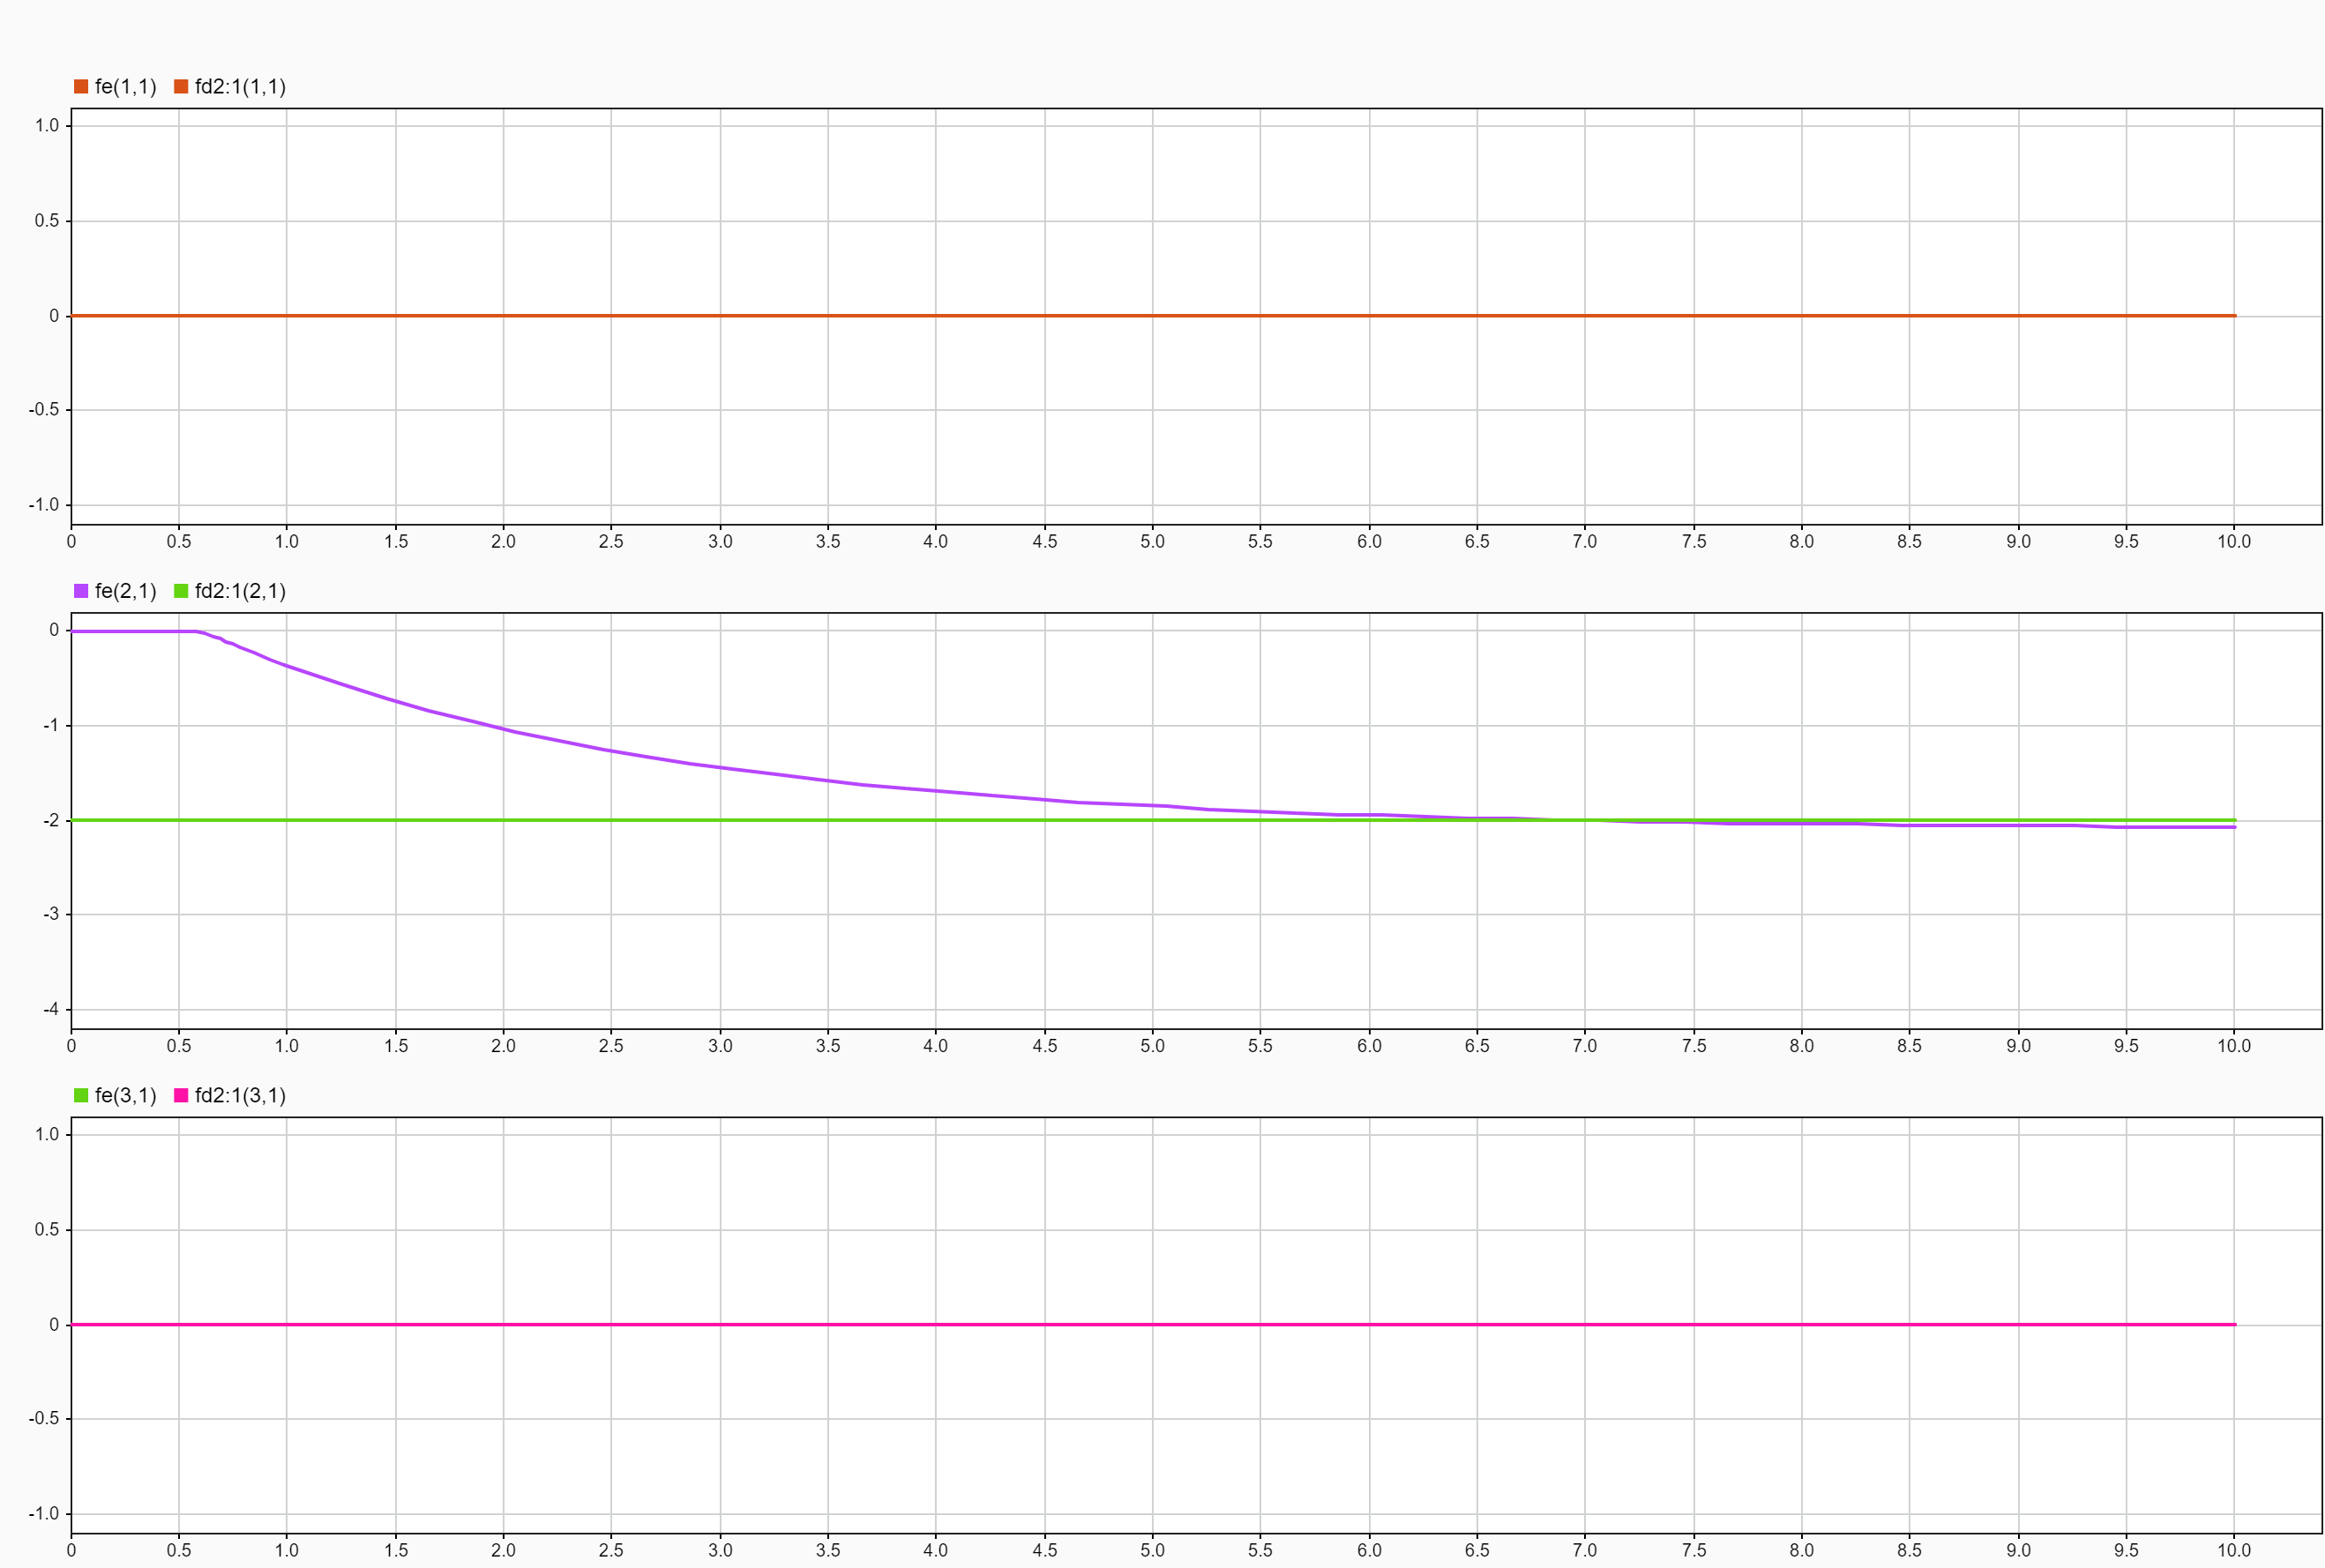
\includegraphics[width=1.2\textwidth]{../Simulink/Images/parallelForce_graph.png}}
    \caption{parallel force/position control}
    \label{fig:parallelForce_graph}
\end{figure}



\end{document}



